\documentclass[10pt,twoside]{article}

\usepackage[tone]{tipa}
%ADDED PACKAGE:
%necessary in order to define fonts
\usepackage{fontspec}
\usepackage{tikz}
\usepackage{times,amsmath,color,xspace,setspace,cgloss4e,arydshln}
\usepackage[round]{natbib}
\usepackage[tipa]{ucs}
\usepackage[utf8x]{inputenc}
\usepackage{graphicx}	%pdftex option clashes with xelatex
\usepackage[text={10cm,17cm}, papersize={15.5cm,23cm}, centering]{geometry}
\usepackage[normalem]{ulem} 

\usepackage[stable]{footmisc}	%	this package lets you put a footnote mark in a
				%	section title.	
% LaTeX was unhappy if this was not loaded last.
\usepackage{gb4e}
%


%%%%%%%%%%%% header
\usepackage{fancyhdr} % customize page header
\pagestyle{fancy}
\renewcommand{\sectionmark}[1]{\markright{#1}}%
\fancyhf{} % clear headers and footers
\fancyhead[LE]{\thepage\hskip0.25em\relax--\hskip0.25em\relax\itshape Jesse Lovegren \& Rebecca Voll\rm}
\fancyhead[RO]{\itshape Relative clause constructions in two Yemne-Kimbi languages --\rm\hskip0.25em\relax\thepage}
%\fancyhfoffset[RO,LE,LO,RE]{0em}
%\renewcommand{\headrulewidth}{0pt}
%\renewcommand{\footrulewidth}{0pt}

% For latext2rtf compatibility comment out
\newenvironment{subexample}{}

%ADDED PACKAGE:
%IPA doesn't work without this one
\setromanfont[Mapping=tex-text]{EB Garamond}
%\setromanfont[Mapping=tex-text]{Essays1743}
\newfontfamily{\ipaFont}[Mapping=tex-text,Renderer=ICU]{Charis SIL}
%\newcommand{\url}[1]{\texttt{#1}}
% Formatting
\newfontfamily\citationfont[FakeBold=2.0]{Charis SIL}
\newcommand{\lmr}{\fontfamily{lmr}\selectfont} % Latin Modern Roman
\newcommand{\lmss}{\fontfamily{lmss}\selectfont} % Latin Modern Sans
\newcommand{\lmtt}{\fontfamily{lmtt}\selectfont} % Latin Modern Mono
%I took this out cause I don't want to spend too much time on searching the font; feel free to send it to me and I'll put it back in!
%\newfontfamily{\purisa}{Purisa}
\renewcommand{\textsl}[1]{\tikz[baseline=(X.base)] \node[xslant=0.2231153] (X) {#1};} % http://stackoverflow.com/questions/1289439/how-do-i-fake-slanted-text-in-latex
\def\ci#1{{\ipaFont #1}}
\def\xci{\textbf}
\def\sn{\textbf}
%\def\gl{}
\newcommand{\gl}[1]{`#1'}
\newcommand{\term}[1]{`#1'}
\def\pl{}
\def\VSP{\vspace{0pt}}
\def\tbf{\textbf}
\newcommand{\cl}[1]{{\sc cl#1}}
%\renewcommand{\s}[1]{\sc \MakeLowercase{#1}}
% citation commands
\newcommand{\citepage}[2]{\citeauthor{#1}~{(\citeyear{#1}:\,{#2})}}
\newcommand{\citepp}[2]{(\citealp{#1}:\,{#2})}
\newcommand{\citeA}[1]{\citeauthor{#1}~(\citeyear{#1})}
\newcommand{\citeps}[2]{\citeauthor{#1}{'}s~{(\citeyear{#1}:\,{#2})}}
\newcommand{\cites}[1]{\citeauthor{#1}'s~(\citeyear{#1})}
\newcommand{\citeyearpage}[2]{\hbox{(\citeyear{#1}:\,{#2})}}
\newcommand{\citeslashpage}[3]{\citeauthor{#1}~{(#2/\citeyear{#1}:\,{#3})}}
\newcommand{\citeslashyearpage}[3]{\hbox{(#2/\citeyear{#1}:\,#3)}}
\newcommand{\citeslashpp}[3]{(\citeauthor{#1},~{#2/\citeyear{#1}:\,{#3})}}
\newcommand{\citeslashA}[2]{\citeauthor{#1}~(#2/\citeyear{#1})}
\newcommand{\citealppage}[2]{\citealp{#1}:\,{#2}}
%\renewcommand{\citep}[1]{(\citealp{#1})}

\newcommand{\mc}[3]{\multicolumn{#1}{#2}{#3}}
\newcommand{\SU}[1]{$^{\text{{#1}}}$}
\newcommand{\su}[1]{$_{\text{{#1}}}$}
\newcommand{\pref}[1]{(\ref{#1})}
\newcommand{\rref}[2]{\pref{#1}--\pref{#2}}
\newcommand{\sref}[1]{Section \ref{#1}}
\newcommand{\tref}[1]{Table \ref{#1}}
\newcommand{\fref}[1]{Figure \ref{#1}}
\def\elicited{$^\diamond$}
% Miscellaneous symbols
\def\goesto{$\rightarrow$\hspace{2pt}}
\def\bad{\hspace{-5pt}*}
\def\til{\raise.17ex\hbox{$\scriptstyle\mathtt{\sim}$}}	% tilde for reduplicant boundary

% Tones
\def\ML#1{#1\symbol{"1DC6}} % more elegant definition taking advantage of Charis SIL & XeTeX
\def\HM#1{#1\symbol{"1DC7}}
%\newcommand\HM[1]{\ipaclap{#1}{\rotatebox{180}{\emph{\raisebox{-.76em}{\texthighrise{}}}}}}
%\newcommand\ML[1]{\ipaclap{#1}{\rotatebox{180}{\emph{\raisebox{-.76em}{\textlowrise{}}}}}}
\newcommand\MH{\texthighrise}
\def\LM{\textlowrise}
\def\LL{\textdoublegrave}

% Special characters
\def\KrnF{f\kern0.8pt{}} % for an f preceding a vowel with a left-spilling diacritic
%\newcommand\Lbi{\ipabar{\tipaencoding \`\i}{.5ex}{1.1}{}{}}
\newcommand\Lbi{\ipabar{\ipaclap{\i}{\rotatebox{0}{\emph{\raisebox{.06em}{\`{}}}}}}{.5ex}{1.1}{}{}}
\newcommand\Hbi{\ipabar{\ipaclap{\i}{\rotatebox{0}{\emph{\raisebox{.06em}{\'{}}}}}}{.5ex}{1.1}{}{}}
%\newcommand\Hbi{\ipabar{\tipaencoding \'\i}{.5ex}{1.1}{}{}}
\newcommand\Mbi{\ipabar{\tipaencoding \=\i}{.5ex}{1.1}{}{}}
\newcommand\MLbi{\ipabar{\ipaclap{\i}{\rotatebox{180}{\emph{\raisebox{-.76em}{\textlowrise{}}}}}}{.5ex}{1.1}{}{}}
\renewcommand{\i}{ı}
\def\@{ə}
\def\eh{ɛ}
\def\oo{ʊ}
\def\aw{ɔ}
\def\ih{ɩ}
\newcommand\bi{\ipabar{\tipaencoding \i}{.5ex}{1.1}{}{}} 
\def\ng{ŋ}
\newcommand\tp[1]{\textipa{#1}}	% needed to put accent over \ng
\def\ny{ɲ}
\def\mj{mj}
\def\dzh{dʒ}
\def\sh{ɕ}
\def\tch{ʨ}
\def\j{j}
\def\hw{\textturnh}
\def\bu{\textbaru}
\def\bdi{\textbari}
\def\?{\textglotstop}
\def\-{\textsubtilde}
\def\st{\textsubtilde}
\def\alp{{\greektext a}}
\def\mf{\textltailm}
\def\t{\texttoptiebar}
\def\var{\kern 0em\lower .7ex\hbox{\~{}}\kern .04em}

% use Charis SIL in ILGs
\renewcommand*\eachwordone{\ipaFont}

%ADDED COMMAND:
%for comments in color:
\newcommand{\comment}[1]{\textcolor{blue}{\emph{#1}}}

% Section headers
% Remove for conversion
%\makeatletter
%\renewcommand{\section}{\@startsection
%{section}
%{0}
%{0pt}
%{-\baselineskip}
%{3pt}
%{\large \bf}}
%\makeatother
%
%\makeatletter
%\renewcommand{\subsection}{\@startsection
%{subsection}
%{1}
%{0pt}
%{-\baselineskip}
%{3pt}
%{\bf}}
%\makeatother
%
%\makeatletter
%\renewcommand{\subsubsection}{\@startsection
%{subsubsection}
%{1}
%{0pt}
%{-\baselineskip}
%{3pt}
%{\it}}
%\makeatother
%
%\makeatletter
%\renewcommand{\paragraph}{\@startsection
%{paragraph}
%{1}
%{0pt}
%{-\baselineskip}
%{3pt}
%{}}
%\makeatother

% For paragraphs as subsubsubsections
\setcounter{secnumdepth}{3}


% For the double-width lines in the table
\def\Hline{\hline}
% Commenting our for RTF
%\newdimen\arrayruleHwidth
%\setlength{\arrayruleHwidth}{1pt}
%\makeatletter
%\def\Hline{\noalign{\hrule \@height \arrayruleHwidth}}
%\makeatother 


%This keeps the footnotes from indenting
\makeatletter \renewcommand\@makefntext[1]{%
\parindent 1em%
\noindent \@makefnmark\,#1}
\makeatother

%\doublespacing

%\def\title{Relative clause constructions in two Yemne-Kimbi languages}

\AtBeginDocument{%
	\pdfpageheight = \paperheight
	\pdfpagewidth = \paperwidth
	}



\usepackage{hyperref}
% get rid of borders on links
\hypersetup{colorlinks=false,
	pdfborder = {0 0 0},
}
%To anonymize
%\def\Good{the first author\xspace}
%\def\Lovegren{the second author\xspace}
%\def\Voll{the fifth author\xspace}

%To not anonymize
\def\Good{Good\xspace}
\def\Lovegren{Lovegren\xspace}
\def\Voll{Voll\xspace}

\title{Relative clause constructions in two Yemne-Kimbi languages}
\author{Jesse Lovegren and Rebecca Voll}
\date{{
%\purisa 
last updated \today}}
\begin{document}

%ADDED THIS
%creates small caps
%\newfontfamily\scshape[Letters=SmallCaps, Numbers=Uppercase]{Hoefler Text}

\maketitle

\section{Introduction\footnotemark}\label{secIntroduction}
%
\footnotetext{This work was made possible by support from 
NSF grant BSC-0853981, University at Buffalo College of Arts and
Sciences Humanities Institute, Leiden University Fund and Leiden University Centre for Linguistics at Leiden University.
Thanks to Jeff Good for
helpful comments on earlier drafts of this paper. We owe a special
debt to a large number of language consultants who provided data,
foremost of which are Kang Protus (Biya), Nchang Adeline (Abar), Ngong Belta (Munken) and
Yung Donatus Kungmba (Mundabli).
Mungbam data were collected by Lovegren during two field trips,
in 2010 and 2012, totaling seven months. Access to Ngun consultants
was limited in the first trip and non-existent in the second trip,
so Ngun data is rather sparse compared to data from the other
dialects. Mundabli data were collected
by Voll during three field trips,
in 2008, 2009 and 2012, totaling eight months.
}
%
The purpose of the present paper is to describe basic facts about
relative clause constructions in two related languages spoken at the northern
edge of the Cameroonian Grassfields, Mungbam and Mundabli. Though
the two languages are not mutually intelligible, there is considerable
contact between their speakers, and basic as well as non-trivial
formal properties relevant to relative clause constructions are to
a large extent isomorphic in the two languages. We therefore find
it profitable to present an analysis which is unified in its formal
analysis of the relative construction, but more ramified where
individual differences are to be noted.

%
%
\subsection{Organization of the paper}
%
In the remainder of~\sref{secIntroduction},
we give basic geographic information about the two languages
and where they are spoken~(\sref{secGeographic}),
and outline their major typological properties,
especially those relevant to the analysis of relative clause
constructions~(\sref{secTypological}).
%
In sections~\ref{secMungbam}--\ref{secMundabli}, we proceed to
a more detailed description of the properties of relative clause constructions
for Mungbam, and then for Mundabli. 
These sections focus on
parallel themes: the linear order of the relative clause with respect
to the head noun, and with respect to other nominal modifiers;
properties of the relativizer and comments on possible grammaticalization sources;
the status of what are typically referred to as resumptive pronouns, 
or ``representative nominals,'' as we call them here, and
the accessibility of different types of formally distinct grammatical
%
%
relations to relativization.\footnotemark\/
%
\footnotetext{Here we refer to the concept
developed in the works of~\cite{keenan:1977,keenan:1979a,keenan:1979b}.}
%
Section~\ref{secDiscussion}
concludes the paper with a discussion summarizing the key points of
similarity and difference between the two languages, and draws attention
to the most typologically interesting points.
%
\subsection{Language background}\label{secLanguageBackground}
%

\subsubsection{Geographic and sociolinguistic background}\label{secGeographic}
%

Mungbam and Mundabli are both spoken within a small part of Cameroon's
Northwest Region near the Nigerian border known as Lower Fungom. As can be seen from the map
in figure~\ref{lfmap} \citepp{dicarlo:2011}{57}, no more than 10km separates
Mundabli from the most distant of the Mungbam villages. 

The acronym ``{Mungbam}'', 
associated with ISO~693-3 code~[mij], is used to refer to the speech varieties used
predominantly
in the villages of \uline{Mu}nken, \uline{Ng}un, \uline{B}iya,
\uline{A}bar and \uline{M}issong (see~\fref{lfmap}). 
There is no locally recognized name to refer to
these five more or less mutually intelligible speech varieties,
and no realistic chance that Mungbam speakers would agree
to a name which groups the five villages together (see~\cite{ideologies}
for discussion on this point).
%At the time of writing, there is also no acceptable
%ISO-recognized name associated with the ISO~639-3 code associated
%with Mungbam, [mij].\footnotemark\/
%%%
%\footnotetext{This may change by the time this article goes to press.}
%%
Mundabli is the name of the speech variety used in the village of the
same name in Lower Fungom. Along with the dialects spoken in the
villages of Mufu and Buu (see fig.~\ref{lfmap}), it is temporarily
referred to with the language name~``Ji'', associated with ISO~693-3
code~[boe].
%

The genetic classification of the two languages is uncertain at this point.  
Although it is uncontroversial
to consider both as Bantoid languages under the Benue-Congo branch of Niger-Congo,
the nature of their relationship to neighboring languages
and to each other will remain uncertain until further comparative work
is undertaken. For the meantime, the referential classification term
``Yemne-Kimbi'', comprising
the Lower Fungom languages Mungbam, Ji, Koshin, Fang and Ajumbu, has been proposed by
\cite{good:inprep} to replace the presently-unsupported genetic label ``Western Beboid.''
This point notwithstanding, however, our experience studying the two
languages has made it clear that the languages overlap considerably
in their overall grammatical structure. What is uncertain is the extent
to which this overlap is due to contact, rather than common inheritance.

As is shown in~\fref{lfmap}, there are non-Yemne-Kimbi languages spoken in close
vicinity to both Mungbam and Mundabli. The most relevant of these is
the Beboid language Naki [mff], which is in especially tight contact
with both languages. The Mungbam villages Biya and Ngun, for example,
are as close to the Naki-speaking village Small Mekaf as they are
to any other Mungbam-speaking village. Likewise for Mundabli, the
closest village is not a Ji-speaking village, but the Naki-speaking
village Mashi. Various West and Central Ring languages are spoken
in and around Lower Fungom. North of Lower Fungom on the Cameroonian
side of the Nigeria-Cameroon border are found Jukunoid languages, including
Yukuben, Akum, Beezen and Baazem (not shown in~\fref{lfmap},
but see~\cite{breton:1993}).
%%
\subsubsection{Typological background}\label{secTypological}
%%%%%%%%%%%%%%%%%%%%%%%%%%%%%%
Basic information about the grammatical systems of Mungbam and Mundabli,
to the extent they were understood at the time of publication, is presented
in~\cite{good:inprep}. Since our understanding of the two languages has evolved
since the time of publication of that article, any conflicting information
presented in the present work should be considered as superseding the
earlier article.

Both languages are rather complex phonologically. Vowel inventories
are relatively large, and vowels in Mundabli contrast for pharyngealization.
Both languages contrast four level tones in addition to
contour tones, and make extensive use of tone in their verbal
morphologies. Words tend to be disyllabic in Mungbam, and mostly
monosyllabic in Mundabli.

Both languages have well-articulated systems of noun class agreement:
All nouns are lexically associated with a noun class, 
and modifiers of the noun exhibit concord
which is controlled by the noun class of the head noun.
The two languages differ in that while noun class is for the
most part overtly marked on nouns in Mungbam via prefixation,
noun class in Mundabli is instead to a considerable extent
``covert'', as it is for the most part only observable via
its ability to control concord agreement.\footnote{See~\citepage{good:kwanoun}{\S4}
for a discussion, with specific reference to Mundabli and Mungbam}
Table~\ref{tblPrefix} illustrates this point, showing some cognate
forms from different noun classes in Mundabli and the Munken
dialect of Mungbam. 

%%
%Information about constituent order within the noun phrase
%will be given separately for each language, since minor differences
%between the languages make a concise but general description
%difficult.
\begin{table}[h!]
\centering
\begin{tabular}{llllll}
\Hline
Mundabli	&	Munken		&	gloss		&	Mundabli&	Munken		&	gloss			\\
\hline
\ci{gb{\=\aw}}	&	\ci{\'u-kp\H{e}}	&	\gl{\cl3.house}	&	\ci{dz\=\aw}	&	\ci{\'\i-kp\H{e}}	&	\gl{\cl4.houses}	\\
\ci{y\H{\ih}}	&	\ci{\'\i-dz\H{\eh}h\eh} &	\gl{\cl3.eye}	&	\ci{y\H{\ih}}	&	\ci{\'a-dz\H{\eh}h\eh}	&	\gl{\cl7a/\cl6.eyes}	\\
\ci{k\=\oo}		&	\ci{\`a-k\ML{\@}f\@}	&	\gl{\cl7/\cl12.bone}	&	\ci{k\=\oo}	&	\ci{b\=\i-k\ML{\@}f\@}	&	\gl{\cl8.bones}		\\	% 26-may-2008 jcg tape
\ci{\dzh\v{u}}	&	\ci{\`\i-b\'e}	&	\gl{\cl9.goat}	&	\ci{\dzh\H{u}}	&	\ci{\'\i-b\H{e}}	&	\gl{\cl10.goat}		\\
\Hline
\end{tabular}
\caption{Forms illustrating the loss of segmental noun class prefixes in Mundabli vs.
their retention in Munken}\label{tblPrefix}
\end{table}
%%
%\footnotetext{The cognacy of these two forms may not seem apparent at first glance,
%but they are most likely both descended from an earlier form~\ci{*\`\i-bu} (cf.~Missong~\ci{\`\i-b\'u}),
%where Mundabli has undergone palatalization of the labial consonant (see \cite{ohala:1978}
%for discussion of this type of sound change), which may also be seen in the correspondence:
%\ci{\dzh\v{\i}}~(Mundabli) -- \ci{\`\i-b\'\i}~(Munken)~\gl{\cl9-dog}.}
%%

In both languages, verbs may be divided
on the basis of tonal alternations
into three different conjugation classes,
labeled \gl{{\sc a}}, \gl{{\sc b}}, and \gl{{\sc c}}.
%%
Cognate verbs in the two languages tend
to fall into the same conjugation class.
%%
Verbs inflect
via tone changes and stem vowel mutations,
the latter of which are conditioned by
a perfective/imperfective aspectual distinction.
Tense marking is produced by a combination of
verb stem changes and overt preverbal tense markers.
Both Mundabli and Mungbam distinguish
four degrees of remoteness in the past (glossed
{\sc p0}, {\sc p1}, {\sc p2}, and {\sc p3} here). Mungbam has one
future tense, while Mundabli has two (glossed {\sc fut1} and {\sc fut2}).
In Mungbam, tone changes in the verb encode a four-way
formal distinction: between perfective and imperfective
aspect on one dimension, and between 
realis and irrealis mood on the other (see~\tref{tblConjugation}).
The latter distinction is mostly a formal one, as the
category ``Irrealis'' has an idiosyncratic membership
 in Mungbam: subjunctive, jussive,
remote past, and one type of negation construction, but
not future and not a second type of negation construction. 
The tonal morphology of Mundabli verbs is a bit
more complicated, and cannot be succinctly summarized
here (but see~\cite{voll:verbs} for details).
%
\begin{table}[h!]
\centering
\begin{tabular}{l|lll}
\Hline
        &                       &       {\sc pfv}       &       {\sc ipfv}      \\
\hline
{\sc a}     &       {\sc realis}    &       \ci{\`x}             &       \ci{\`x} $+$ {\sc abl}       \\
        &       {\sc irr}       &       \ci{\={x}}           &       \ci{\={x}} $+$ {\sc abl}     \\
\hline
{\sc b}     &       {\sc realis}    &       \ci{\H{x}}           &       \ci{\^x} $+$ {\sc abl}       \\
        &       {\sc irr}       &       \ci{\ML{x}}          &       \ci{\'{x}} $+$ {\sc abl}     \\
\hline
{\sc c}      &       {\sc realis}    &       \ci{\^x}             &       \ci{\^x} $+$ {\sc abl}       \\
        &       {\sc irr}       &       \ci{\'{x}}           &       \ci{\'{x}} $+$ {\sc abl}     \\
\Hline
\end{tabular}
\caption{Verb conjugation in Mungbam. Tone diacritics are interpreted as
follows: \ci{\`x} $=$ L, \ci{\={x}} $=$ M, \ci{\ML{x}} $=$ ML, \ci{\'{x}} $=$ H, \ci{\^{x}} $=$ HL,
\ci{\H{x}} $=$ S(uperhigh). {\sc abl}$=$ `ablaut'.
On disyllabic verbs, the patterns are identical, with the pitch modulation
spread across the two syllables.}
\label{tblConjugation}
\end{table}
%

%Presentation of inflectional paradigms for verbs is not
%convenient here, given space limitations, so glosses 
%indicating which of the possible inflected forms of a verb
%are observed will have to be taken at face value.

Basic constituent
order in both languages is SV/SVO, though arguments are frequently dislocated
to different positions within the clause for focus-marking.
More specifically, the position immediately after the verb (IAV) is
considered a structural
focus position in both languages. This means that VS constituent
order is observed in subject-focus constructions, and OV constituent
order is observed in object-defocalisation constructions.
In Mungbam, a productive process of verbal reduplication
is available for the encoding of verum focus (contrastive
or assertive focus on the truth value of a clause).
Reduplication is however under partial grammatical control (cf.~\citepage{hyman:1984}{243})
when certain marked constituent orders are observed, as
well as in relative clauses (see
\sref{secMungbamFocus}).

Both languages make extensive use of serial verb constructions
in which all of the verbs form a continuous block
in the middle of the clause, without any intervening arguments.
In this paper the term ``verbal complex,'' taken over
from \cite{kiessling:2011},
refers to this
continuous block of one or more verbs.

With some minor differences, the two languages have broadly similar
systems for formally marking different types of grammatical relations, with
the following formally distinct possibilities available:
%%
\begin{itemize}
\item	Subject (\o-marked, normally appears before the verb). Some preverbal subject pronouns differ from 
	postverbal object pronouns.
\item	Object (\o-marked, normally appears immediately after the verb)
\item	Comitative (preceded by particle glossed~{\sc com})
\item	Dative (optionally preceded by a general-purpose preposition, followed by a particle glossed~{\sc dat})\footnotemark
\item	Locative (optionally preceded by a general-purpose preposition, followed by one of several possible postpositions)
\item	(Genitive) (\o-marked, follows the head noun)
\end{itemize}
%
\footnotetext{
	The comitative is so called because it is prototypically used to encode accompaniment. It
	is also used with instrumental function. The dative is so called because it is prototypically
	used to encode recipients. It is also used with benefactive function.
	We employ the terms ``comitative phrase'' and ``dative phrase'' as necessary to
	refer to a noun phrase together with its associated comitative- or dative-marking morphology.

	Dative-marked arguments in Mungbam and Mundabli overlap in function somewhat with
	arguments licensed by reflexes
	of the verbal suffix \ci{*-\ih{}l-} in Narrow Bantu
	languages, commonly called ``applicative,'' though called ``dative'' by \citepage{schadeberg:2003}{74}.
	In referring to the grammatical function in
	Mungbam and Mundabli, we prefer the latter term,
	 since ``applicative'' is typically associated
	with head-marking strategies for encoding grammatical roles, while ``dative'' 
	is typically associated with dependent-marking strategies.
}
%%

We will occasionally refer to these grammatical relations in
our discussion of accessibility.
%%%%%%%%%%%%%%%%%%%%%%%%%%%%%
\begin{figure}[p]
\centering
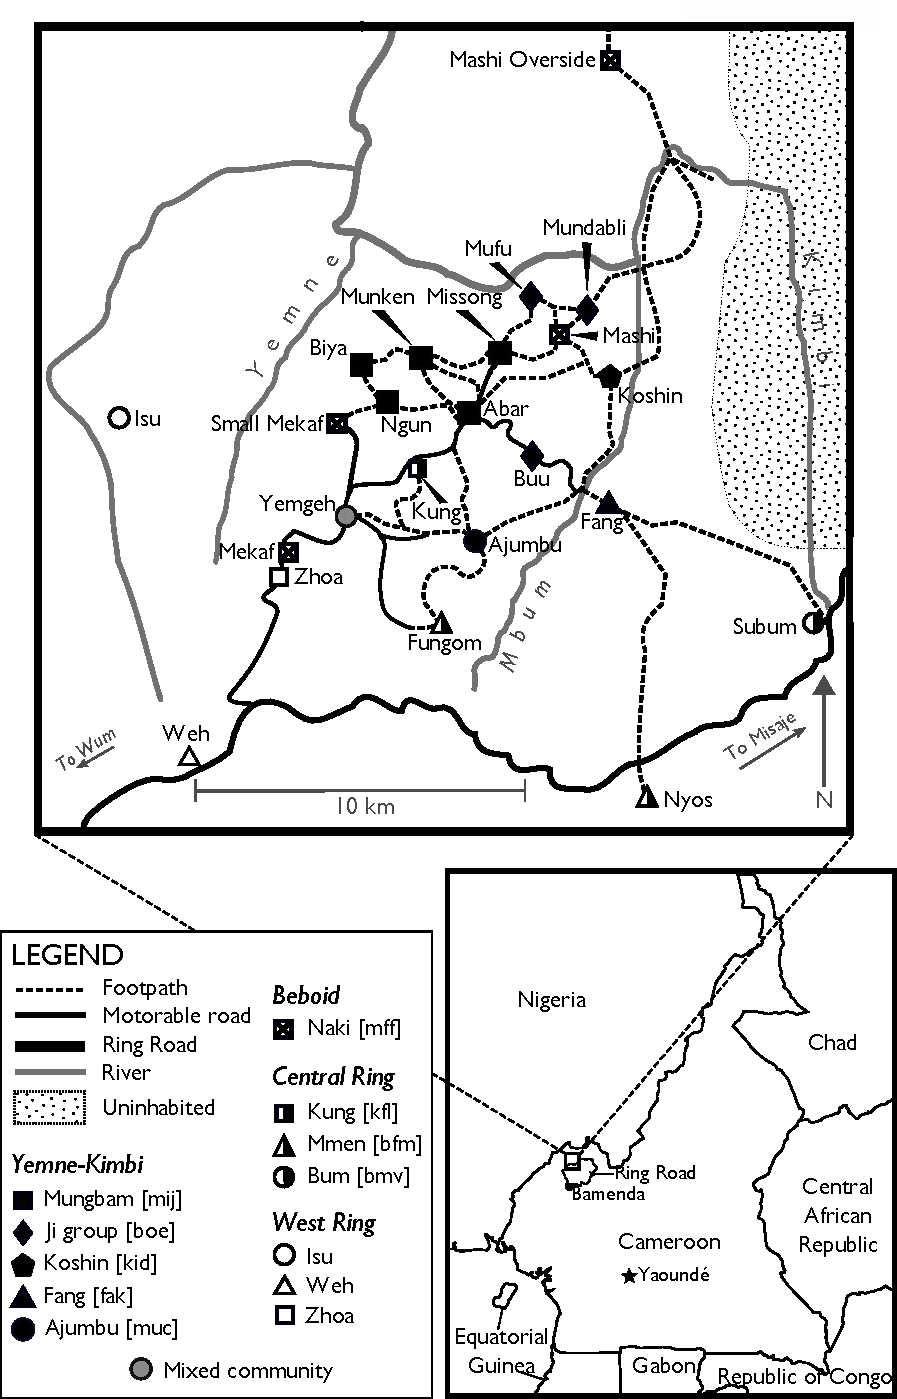
\includegraphics[width=10cm]{LowerFungomLanguagesMap.pdf}
\caption{Lower Fungom and surrounding area \citep{good:inprep}.}\label{lfmap}
\end{figure}%%%

\subsection{Notes on terminology and transcription}\label{secTerminology}

\fbox{Transcription} symbols used in the examples are mostly consistent
with the corresponding IPA symbols, with a few minor exceptions. 
The use of the \ci{[\textsubumlaut{x}]} diacritic, normally reserved to indicate breathy voice,
is used to indicate what has been described as pharyngealisation of
vowels in Mundabli. 
Also, the symbol \ci{[y]} indicate a palatal glide in Mundabli. 
In Mungbam a palatal glide is indicated by the IPA symbol \ci{[j]}. Additionally, we prefer to use the now outdated 
%symbol~\ci{[\,\scalebox{1.5}{{\ih}}\,]} rather than the currently-recommended~\ci{[\,\scalebox{1.5}{{\tp{I}}}\,]}
symbol \ci{[\ih]} rather than the currently-recommended \ci{[ɪ]} 
to transcribe a high, front, unrounded root-retracted vowel, simply
for the reason that when tone diacritics are included,
the latter symbol is easily confused with
%dotless~\ci{[\,\scalebox{1.5}{{\i}}\,]}. 
dotless \ci{[{\i}]}. 
%In Mungbam, the vowel transcribed with this
%symbol is lower than cardinal~[\,\ci{\ih}\,] (and lower than
%Mungbam /e/), though in Mundabli
%it is high for most speakers.

For terminological convenience, we use the term~\gl{head nominal}
to refer to the head of a noun phrase which contains a relative
clause, and the term~\gl{representative of the head nominal}
(or simply~\gl{representative nominal}),
to refer to a noun {or pronoun} coreferent with the head nominal which
occurs inside of
the relative clause itself. 
Both terms are due to~\citepage{lehmann:1986}{664,673}.
We also use the term~\gl{matrix NP}, due to~\citepage{andrews:2007}{206},
to refer to the noun phrase
headed by the head nominal. Likewise, we use~\gl{matrix clause} to
designate the clause containing the matrix NP. Since a discussion of noun class concord
figures prominently in several places in this paper, we use
the term~\gl{concordant} as a short way of referring to a
grammatical particle, viz. a relativizer, which shows noun class concord
with the head nominal. Likewise,~\gl{non-concordant} will designate a
grammatical particle which does not show concord.

In examples, we enclose relative clauses in square brackets, and indicate
head nominals and their representatives within the relative clause with
underlining. In~\sref{secMungbam}, a name in parentheses following the free translation refers
to the dialect from which the example has been taken.
Examples with no such annotation are Mundabli examples.

%\comment{Where do we explain the glossing abbreviations?}

One final comment concerns the source of the example sentences. %
Example sentences drawn from naturally-occurring speech are generally
to be preferred. However, an elicited sentence is often the best way
to clearly exemplify a particular type of structure to the audience
of linguists.
At a more practical level, elicitation is the most convenient way
for a visiting field linguist to test hypotheses that they
develop through the examination of texts, and is often
the only sensible way to do so, given time constraints. Examples used in this
paper, then, come from both elicited and naturally-occurring speech.
Elicited sentences are indicated by a~\elicited~symbol in the free
translation.

%

\section{Mungbam}\label{secMungbam}
%
\subsection{Introduction}\label{secMungbamIntro}
%

Data from Mungbam will be drawn freely from all five
varieties, with the understanding that the same facts apply
to each variety, except where otherwise mentioned.
We first consider superficial properties of the relative
clause construction, including the order of the relative
clause with respect to other nominal modifiers~(\sref{secMungbamOrder}).
We then consider properties of the relativizer, including its likely
historical source~(\sref{secMungbamRelativizer}).
Section~\ref{secMungbamRepresentative} concerns the
representative nominal, and~\sref{secMungbamAccessibility}
discusses the accessibility of different grammatical
relations to relativization.
Finally,
section~\ref{secMungbamFocus} compares the possibilities
for marking various clause-level properties in
main and relative clauses. Special attention is given
to focus-marking possibilities.
%
\subsection{Basic order of constituents in the NP}\label{secMungbamOrder}
%
The unmarked constituent order within NP's in Mungbam is such that
the head noun is initial. The head noun may be modified by
possessive pronouns, demonstratives, adjectives, numerals, the
definite determiner, and relative clauses, all of which,
save the relative clause,
show some form of concord with the noun class of the head noun
in all Mungbam varieties.\footnotemark\/
%
\footnotetext{Concord on possessive pronouns is, however,
significantly eroded. Only a two-way tonal distinction
is realized on pronouns, depending on whether the possessum
noun class is one of \{1,5,9\}, or some other class.}
%
The order of certain other modifiers of
the head noun is as in~(\ref{constOrder}), exemplified in~(\ref{mg01}).
Adjectives and numerals, which are for the most part formally
identical to nouns, have a more variable ordering with respect
to other nominal modifiers, so they cannot be easily incorporated
into the schema given in~(\ref{constOrder}).
Since the relative clause appears after the head nominal, but
before the definite determiner,
as in~(\ref{mg01}), it is rather straightforward to argue that
the relative clause is internal to the matrix NP.
%
\begin{exe}
\ex {\sc N} -- {\sc Poss} -- {\sc Dem} -- {\sc Rel} -- {\sc Det}	\label{constOrder}	%	exception in ngun 8-apr-2010 2v
\ex \gll \uline{\'\i-s\HM{\eh}h{\eh}} m\'{\@} j\^{\eh}n n\'{\@} $[$\H{\ny}-\ny\'{\eh} m\={e} \ny\`{\eh}$]$ j\={\eh}	\\
\cl4a-place {\sc 1sg.poss} {\sc \cl4}a.{\sc dem.prox} {\sc rel} \cl6a-water \cl6a.{\sc det} ({\sc a})stay.{\sc pfv} {\sc cl4.det}		\\
\glt \elicited``This my place where there is water\dots'' (Munken)\footnotemark\label{mg01} %104v
\end{exe}
%
\footnotetext{Glossing abbreviations are as follows:
\\
\begin{centering}
\begin{tabular}{llll}
\Hline
a,b,c	&	verbal conjugation class	&	\cl1\dots19(a)	&	noun class	\\
{\sc adj}&	adjectivizer			&	{\sc ass}	&	associative	\\
{\sc aug}&	augment				&	{\sc cop}&	copula			\\
{\sc com}	&	comitative		&	{\sc comp}&	complementizer	\\
{\sc consec}&	consecutive			&	{\sc dem}&	demonstrative	\\
{\sc det}&	definite determiner		&	{\sc dist}&	distal	\\
{\sc ds}&	dummy subject			&	{\sc dsf}&	disfluentive (cf.~\citepage{good:2009}{\S4})	\\
{\sc excl}&	exclamatory			&	{\sc foc}&	focus-field form	\\
{\sc frust}&	frustal			&	 {\sc fut, fut1\dots2}&	future	\\
{\sc ideo}&	ideophone			&	&	\\
{\sc ipfv}&	imperfective			&	{\sc irr}&	irrealis	\\
{\sc loc}&	locative			&	{\sc neg}&	negative	\\
{\sc nmlz}&	nominalizer			&	{\sc poss}&	possessive	\\
{\sc prep}&	preposition			&	{\sc prf}&	perfect		\\
{\sc p0\dots3}&	past tense			&	{\sc pst}&	past tense	\\
{\sc prox}&	proximal			&	{\sc pro}&	proform		\\
{\sc red}&	reduplicant			&	{\sc rel}&	relativizer	\\
{\sc subd}&	subordinator			&	{\sc top}&	topic-field form; topic		\\
{\sc vent}&	ventive				&	{\sc vfoc}&	verum focus	\\
\Hline
\end{tabular}
\end{centering}

Verbs not glossed as `{\sc ipfv}' are in their perfective forms. Mungbam verbs
not glossed as `{\sc irr}' are in their realis forms.}
%

Departures from the determiner-final
constituent order given in~(\ref{constOrder})
are found
under different scopal interpretations of definiteness
with respect to other constituents of the NP. While the normal state
of affairs is for either all or none of the information in the NP to
be given a definite interpretation, corresponding to 
either the appearance of the determiner NP-finally or its complete absence,
some cases are possible where the
head nominal is given a definite interpretation, but one of its modifiers
is given an indefinite interpretation.
Example~(\ref{mg02}), for example, where the relative clause follows
the definite determiner, is felicitously uttered in a context where
the listener is familiar with the group of fowls being discussed, 
and familiar with the set of red fowls within that group, and also
familiar with the fact that some fowls within the group fell, 
but did not know beforehand that the fowls having fallen were the red
ones.
%
\begin{exe}
\ex \gll \uline{\'\i-\sh\H{\eh}} j\={\eh} n\'{\@} $[$\uline{\'{\i}} gb\`e$]$ \'\i-bw\'{\ih}ns\'{\@} j\={\eh}	\\
\cl10-fowl {\sc \cl10.det} {\sc rel} \cl10 ({\sc a})fall \cl10-red {\sc \cl10.det}	\\
\glt \elicited``The fowls which fell are the red ones.'' (Munken)	\label{mg02}
\end{exe}
%

\subsection{The relativizer}\label{secMungbamRelativizer}
%

%%
In the Munken examples~(\ref{mg01})--(\ref{mg02}), the relativizer, which
immediately precedes and introduces the relative clause, does not show concord
with the head nominal. In all of the Mungbam varieties, except for Biya (to be
discussed below), the relativizer is non-concordant.
These (non-)agreement facts are noteworthy because they not only
separate Mungbam from other Grassfields languages further to the South,
which have concordant relativizers,\footnotemark\/
\footnotetext{cf. for Isu (Ring) \citepp{kiessling:2011}{39,\,passim},
Noni (Beboid) \citepp{hyman:1981}{91}, Bafut (Ngemba) \citepp{tamanji:2009}{96--7}.
Mankon (Bamil\'ek\'e) \citepp{leroy:2007}{415}, and
Ngwe (Bamil\'ek\'e) \citepp{nkemnji:1995}{77}. An exception is 
the Bamil\'ek\'e language Fe{\ci\textraiseglotstop}Fe{\ci\textraiseglotstop} \citepp{chumbow:1977}{289},
which otherwise has lost much of its concord morphology \citepp{hyman:1972}{\S{VII}}.}
but they also can offer a clue
%
%\subsubsection{Grammaticalization sources for the relativizer}
%
about possible grammaticalization sources for the relativizer.
If the relativizer is non-concordant, then it is less likely
that it could have grammaticalized from an element which regularly
shows concord, such as a demonstrative.\footnotemark\/
%%
\footnotetext{A logical possibility is of course that the relativizer
grammaticalized from a concordant form which eventually lost its
concord. However, with the exception of possessive marking, the
concord system of Mungbam quite well-preserved.}
%%
Ruling out the demonstrative as a grammaticalization source
is significant since demonstratives are a common grammaticalization
source for relativizers in African languages \citepp{heine:2011}{706},
and the ``most frequent'' source cross-linguistically \citepp{heine:2002}{115}. 

%XXX\comment{Maybe, point out that Mundabli has both, a non-concordant marker more generally used as subordinator which is probably cognate with the Mungbam non-concordant relative marker and a concordant relative marker?}

\subsubsection{Possible sources for grammaticalization of the relativizer}
%
In Biya, the relativizer \uline{does} show concord with the head nominal. 
In that variety, the relativizer coincides exactly in form with the word~\ci{-n\ih}~\gl{some, another},
which takes a noun class prefix and whose tone is also controlled by the
class of the noun it agrees with.\footnotemark\/ 
Examples are given in~(\ref{mg101}). The only difference between the two
is that the prefix of the relativizer is occasionally omitted in casual
speech, as in~(\ref{mg101c}).%
\footnotetext{It bears a mid tone for agreement with class 1, 5 and 9, nouns, and a high tone
for all agreement with nouns of all other classes.} Since the agreement
facts between the two morphemes are identical, it seems likely that
the relativizer in Biya has grammaticalized from~\ci{-n\ih}~\gl{some, another}.
%
\begin{exe}
\ex \label{mg101}
\begin{xlist}
\ex
\gll \=\i-\sh\={\eh} j\={\i} \`a t\`u-\=a \={\i}-\sh{\=\eh} \`\i-n\={\ih}	\\
\cl9-fowl \cl9.{\sc det} {\sc sbj} ({\sc a})peck-{\sc prf} \cl9-fowl \cl9-other	\\
\glt \elicited``The fowl has pecked the other fowl.'' (Biya)
%\gll \uline{\`u-n\`o} \`u-n\={\ih} $[$N\H{a}{\ng} f\H{\@} s\`el\`{\@} \uline{w\`{\@}}$]$ \`u kp\'u{\til}kp\H{e}	\\
%\cl1-person \cl1-{\sc rel} N. {\sc p1} insult.{\sc pfv} {\sc \cl1.foc} {\sc \cl1.top} {\sc vfoc}{\til}die.{\sc pfv} \\
%\glt ``The man whom Nang insulted died.'' (Biya)
\ex
\gll \uline{\=u-b\'{\i}} \=u-n\'{\ih} $[$\'u-kp\H{\@} k\={\@}-\ng{w\={a}{a}} s\=u kw\'{\i} \'a w\'ah\'a$]$ w\={\ih}	\\
\cl3-year \cl3-{\sc rel} \cl3-house \cl7-book ({\sc a})start.{\sc irr} ({\sc c})enter.{\sc irr} {\sc prep} Zhoa {\sc \cl3.det}	\\
\glt ``The year when the school at Zhoa was opened\dots'' (Biya)
\ex \label{mg101c}
\gll w\v{\@} \uline{k\'{\@}-mj\H{\ih}} n\'{\ih} $[$\'\ny-\sh\^{\i} \'n-d\'e \sh\={\i} l\={e} k\={\@} j\ML{a}$]$	\\
then \cl7-matter {\sc rel} 1sg-({\sc b})want 1sg-({\sc c})talk.{\sc irr} ({\sc a})discuss.{\sc irr} {\sc vent.irr} {\sc \cl7.foc} thus	\\
\glt ``That's the problem that I want to talk about\dots'' (Biya)
\end{xlist}
\end{exe}



In the other dialects, where concord between the relativizer and the head nominal
is not observed, the forms of the relativizer are quite similar, though the forms
of the~\gl{some, other} morpheme tend to vary (see~\tref{tblmg01}), such
that this morpheme is not the most obvious grammaticalization source.
In~\tref{tblmg01} we give forms for two other morphemes which might be
candidates for grammaticalization sources. 

We note that in Abar, the
word translatable as~\gl{(one's) own}, a type of emphatic associative marker,
coincides in segmental form (though
not in tone) with the relativizer. 
%%
The associative marker as a grammaticalization source for the
relativizer is not mentioned in \citepage{heine:2002}{335},
though \citepage{ohori:2011}{641--2} considers it to be a
source ``\dots with clear conceptual-semantic ground\dots''
Such a grammaticalization scenario is claimed for some Chadic languages~(cf.~\citepage{frajzyngier:1996}{\S11}),
and a relativizing particle in Vute (Mambiloid) is treated by \citepage{maxey:1994}{\S3.1}
as being the same as an associative marker.
A more relevant case is the neighboring language Naki,
where formally identical particles serve as both a pre-RC relativizer and an
associative marker (Jeff Good, p.c.).\footnotemark\/
%%
\footnotetext{See~\pref{exNaki}, p.\,\pageref{exNaki} for an example of a Naki relative clause.}
%%

The root of the word meaning~\gl{reason, problem, matter}
in Missong coincides with the relativizer in that language. The root~\ci{-mj\H{V}}
in Biya, Munken, and Ngun also means~\gl{word}\footnotemark\/ (similar forms with that meaning
are attested in Abar and Missong), and it appears to have supplanted
the original term in Ngun and Biya. Biya and Munken retain roots~\ci{k\'{\@}-n\H{o}}, \ci{\'a-\ny\H{\i}}~\gl{thing},
of the same noun class as Abar~\ci{k\'\@-\ny\H\i}.
%This suggests that even it the relativizer in Biya has grammaticalized from
%\ci{-n\ih}~\gl{some, other}, this may be a more recent innovation, since
%it is unlikely that all varieties of Mungbam have an identical grammaticalization
%pathway for the relativizer.
%
\footnotetext{Interestingly, in Munken, a subordinating particle~\ci{mj\H{u}}, clearly
related to~\ci{\'a-mj\H{u}}, is attested in a type of aversive construction,
translatable as~\gl{lest}.}
%
\begin{table}[h!]
\centering
\begin{tabular}{lllll}
\Hline
variety	&	relativizer	&	\gl{some, another}	&\gl{reason}	&	\gl{own} (associative)\\
\hline
Munken	&	\ci{n\'{\@}}		&	\ci{-l\eh}			&\ci{\'a-mj\H{u}}	&\ci{-\ny\@{m\@}}				\\
Ngun	&	\ci{n\'{\ih}}	&	\ci{-ne}			&\ci{k\'{\@}-mj\H{\ih}}	&					\\	%9/11 22-apr-2010
Biya	&	\ci{-n\ih}		&	\ci{-n\ih}			&\ci{k\'{\@}-mj\H{\ih}}	&\ci{-kj\ih}					\\
Abar	&	\ci{\ny\'\i}		&	\ci{-lehe}			&\ci{k\'{\@}-\ny\H{u}} 	&\ci{-\ny{i}}				\\
Missong	&	\ci{n\'a}		&	\ci{-l\eh}			&\ci{k\'\i-n\H{a}}		&\ci{-n\={\@}}			\\	%83v
\Hline
\end{tabular}
\caption{Forms of relativizer, and of three suspected grammaticalization
sources for the relativizer in Mungbam.
Lack of tone marking indicates that the tone of the form depends on the prefix
it bears.}\label{tblmg01}
\end{table}
%

A possible scenario for grammaticalization of the relativizer from a
word meaning~\gl{matter}, which at this point remains speculative, is as follows:
The word translatable as~\gl{reason, problem, matter}, was originally found in all five varieties
in a form close to that observed in Missong or Abar. This form was the original
source for the relativizer in all of the dialects, and possibly was the source
for the emphatic associative marker translated as~\gl{own} in Abar, Missong and Munken.
Since the prefix in the original word was fixed, the relativizer never showed concord
with the head noun, and this prefix was eventually lost. Some time after the grammaticalization
of the relativizer from~\ci{*kV-nV}, the original root meaning~\gl{matter},
was replaced in Biya, Munken, and Ngun by the root whose original meaning was~\gl{word}.
The relativizer in Biya was eventually reanalyzed as an instantiation of the
morpheme~\ci{-n\ih}~\gl{other}.
\citepage{heine:2002}{211--2, 295} note that a word with the meaning~\gl{thing} or~\gl{matter}
tends to be the grammaticalization source for a complementizer, though
no such source is reported for a relativizer. 

In summary, we have identified two of the most likely historical sources
for the relativizer in Mungbam: an emphatic associative marker, and a lexical
item~\gl{thing, matter}. At present it is not clear which of these
is the more likely.
%As will be discussed
%in~\sref{secMungbamFormal}, however, there is little evidence for treating
%relative clauses as instantiating a special clause type with its own
%syntactic properties. 
%
%\comment{quoth WLG p.295: (about THING $>$ complementizer) ``This appears to be an instance of a more
%general process whereby certain generic nouns serving as nominal complements are grammaticalized to markers
%of complement clauses. In many languages, this process has not proceeded beyong an incipient stage where
%it remains controversial whether, or to what extent, the relevant noun constitutes a noun or a clause subordinator;}
%

\subsubsection{Optionality of the relativizer}
%

The presence of the relativizer is optional in Mungbam. There are,
however, differences between different types of relative clauses with
respect to the rate of its omission. While the relativizer is usually
omitted in cleft sentences, it is usually not omitted in non-cleft sentences.
Example~\pref{exAbar124r} shows two repetitions of the same line
in a folk tale told by different speakers, which differ by
the presence vs. the absence of the relativizer. In~\pref{exAbar124ra},
the original telling of the story, the relativizer is omitted
from the cleft construction, and the copula verb is reduced.
In~\pref{exAbar124rb}, a careful repetition of the same line by
a different speaker, the relativizer is present.
%
\begin{exe}
\ex	\label{exAbar124r}
\begin{xlist}
\ex	\label{exAbar124ra}
%%
\gll \v{a} \uline{fw\H{e}} $[$\`u \sh\^o fw\^om l\`an{\`\aw} k\={\aw} m\`{\eh} b\`\i-dz\={a}{\ng} b\={\i} fw\`{\@}mh\={\aw} w\`{\@} \'\i-d\=a{\ng} \`{\i} \ng\={\@}n$]$	\\
{\sc ds.cop} there \cl1 ({\sc b})stay.day.{\sc ipfv} ({\sc b})struggle.{\sc ipfv} ({\sc a})walk.{\sc ipfv} {\sc ipfv}
{\sc com} \cl8-fly \cl8.{\sc det} ({\sc a})disturb {\sc \cl1.foc} {\sc loc.\cl5-}comb \cl5.{\sc det} {\sc loc.}on	\\
\glt ``It's there [i.e. that's why] he is constantly struggling with flies disturbing
him [landing] on his comb.'' (Abar) % 6r 28-apr-2010

%%
\ex	\label{exAbar124rb}
\gll \`a l\H{\eh} \uline{fw\H{e}} \ny\'{\i} $[$\`u \sh\^o fw\^om l\`an{\`\aw} k\={\aw} m\`{\eh} b\`\i-dz\={a}{\ng} b\={\i} \'\i-d\=a{\ng} \`{\i} \ng\={\@}n$]$	\\
{\sc ds} {\sc cop} there {\sc rel} \cl1 ({\sc b})stay.day.{\sc ipfv} ({\sc b})struggle.{\sc ipfv} ({\sc a})walk.{\sc ipfv} {\sc ipfv}
{\sc com} \cl8-fly \cl8.{\sc det} {\sc loc.\cl5-}comb \cl5.{\sc det} {\sc loc.}on	\\
\glt {``It is there that [i.e. that's why] he is constantly struggling with flies on his comb.'' (Abar)} 	%124r
\end{xlist}
\end{exe}
%
%
\subsection{The representative of the head nominal}\label{secMungbamRepresentative}
%

All relative clauses in Mungbam may contain a representative of the
head nominal, though its presence is only mandatory when the representative
nominal functions as the subject of the relative clause.\footnotemark\/
%%
\footnotetext{A similar asymmetry between extracted subject and non-subjects
is reported for Vata (Kru), which requires an overt representative nominal for
subject relatives, but requires its absence for non-subject relatives \citepp{koopman:1986}{361}.}
%%
In a subject relative clause such as~(\ref{mg002a}), a
pronoun will always follow the relativizer.
%

\begin{exe}
\ex	\label{mg002a}
\gll \uline{kp\`oa} n\'a $[$b\H{u} gb\`{\@}$]$ b\=u	\\
five {\sc rel} \cl2 ({\sc a})fall {\sc \cl2.det}	\\
\glt \elicited``The five that fell\dots'' (Missong)	% 42
\end{exe}
%

For all other types of relative clauses, inclusion of the representative
nominal is optional. Example~(\ref{mg03first}) shows two sentences containing
an object relative clause which differ only by the presence or absence
of a representative nominal in the relative clause.
%
%
\begin{exe}
\ex     \label{mg03first}
\begin{xlist}
\ex     \gll \uline{\`mb\`\oo{\ng}} \ny\'{\i} $[$N\H{a}{\ng} h\H{a} l\Lbi{\ng}$]$ {\`\aw} \`u p\'\i\til{p\H{\i}}        \\
\cl1.cow {\sc rel} N. {\sc p1} ({\sc a})look.for {\sc \cl1.det} \cl1 {\sc vfoc}\til{({\sc b})die} \\
\glt \elicited``The cow that Nang looked for died.'' (Abar)      \label{mg03a}
\ex     \gll \uline{\`mb\`\oo{\ng}} \ny\'{\i} $[$N\H{a}{\ng} h\H{a} l\Lbi{\ng} \uline{w\`u}$]$ {\`u}{\footnotemark} \`u p\'\i\til{p\H{\i}}     \\
\cl1.cow {\sc rel} N. {\sc p1} ({\sc a})look.for {\sc \cl1.foc} {\sc \cl1.det} \cl1 {\sc vfoc}\til{({\sc b})die}  \\
\glt \elicited``The cow that Nang looked for [it] died.'' (Abar) \label{mg03b}
\end{xlist}
\end{exe}
%
\footnotetext{The form of the class 1 determiner in Abar is sensitive to the
presence of a preceding vowel.}
%

Example~(\ref{mg030}) contains a relative clause where the representative nominal
may or may not appear as the object of the locative phrase~\ci{\'a\dots m\=\i}~\gl{inside of\dots}.
As~\pref{mg030} shows, locative phrases may be~``stranded'' in relative clauses.
Object-less locative phrases, however, are grammatical in main clauses as well
(see~\pref{exMunkenDresses}, below).
%
\begin{exe}
\ex	\label{mg030}
\gll 
%\`ak\^{\@}{\ng} k\`{\eh} l\H{\eh} \'a-k\H{a}{\ng} {\ny}\H{\ih} bw\c{\H{e}} {\dzh}\`u
%\'\i-l\Hbi\={m} \`{\eh} (\'a) k\={\i} m\={\i} k\`{\eh}  \\
\`ak\^{\@}{\ng} k\`{\eh} l\H{\eh} \uline{\'a-k\H{a}{\ng}} {\ny}\H{\ih} $[$bw{\H{e}} {\dzh}\`u
\'\i-l\Hbi\={m} \`{\eh} \'a (\uline{k\={\i}}) m\={\i}$]$ k\`{\eh}  \\
\cl7.{\sc dem.prox} {\sc \cl7.det} {\sc cop} \cl7-pan {\sc rel} \cl2 ({\sc a})put.{\sc ipfv}
\cl4a-nkwi.bark \cl4a.{\sc det} {\sc prep} {\sc \cl7} {\sc loc.}in {\sc \cl7.det}   \\
\glt \elicited``This is the dish that nkwi bark is put
inside of.'' (Abar)
\end{exe}
%

In the case of comitative and dative relatives, if the representative nominal is
omitted from the relative clause, then so must the comitative or dative marker
itself (\ref{mg031}). %
\begin{exe}
\ex	\label{mg031}
\gll \=m-f\H{\@} ts\Hbi{n{\til}ts\HM{\aw}\ng\aw} \uline{\'u-\sh\H{\eh}} n\'{\@} $[$N\H{a}{\ng} f\H{\@}
k\`{\@}m \'\i-\sh\H{\eh} j\={\eh} (b\={\@} \uline{w\`u})$]$	\\
1sg-{\sc p1} {\sc vfoc}\til{see} \cl3-knife {\sc rel} N. {\sc p1} slaughter \cl10-fowl
\cl10.{\sc det} ({\sc com} \cl3)	\\
\glt \elicited``I did see the knife that Nang slaughtered the fowls (with it).'' (Munken)
\end{exe}
%

When the head nominal refers to a place where the event described by the relative clause
took place, the relative clause may optionally contain a locative phrase translatable
as~\gl{there}, as in~(\ref{mg032}).
%
\begin{exe}
\ex	\label{mg032}
\gll \=m-f\H{\@} ts\Hbi{n\til{ts\HM{\aw}\ng\aw}} \uline{\'\i-s\H{\eh}h\eh} n\'{\@} $[$N\H{a}{\ng} f\H{\@}
k\`{\@}m \'\i-\sh\H{\eh} j\={\eh} (\uline{\'a f\=e})$]$	\\
1sg-{\sc p1} {\sc vfoc}\til{({\sc b})see} \cl5-place {\sc rel} N. {\sc p1} ({\sc a})slaughter \cl10-fowl \cl10.{\sc det} (there)	\\
\glt \elicited``I did see the place that Nang slaughtered the fowls (there).'' (Munken)	%104v
\end{exe}
%

%%
The conditions on the appearance of a representative nominal
within a relative clause exactly parallel the conditions on the presence
of overt arguments in main clauses.
Just as subject relative clauses are the only type of relative clause which
must contain a representative nominal, subjects are the only argument
which is not omissible from a main clause.
The behavior of comitative and dative arguments is also parallel: in
both relative and main clauses, a comitative or dative argument may be
omitted, provided that the comitative/dative
%
marker is itself omitted. Examples \rref{exMunkenVegetables}{exBiyaWater}
show main clauses with an omitted object, locative complement, and dative,
respectively.
%
%In example~(\ref{mg04}), the second clause contains a notionally transitive
%verb, but no object. The sentence is grammatical, however, because the
%object of the transitive verb~\ci{gj\eh{l\@}}~\gl{cook} can be easily inferred
%from the context.
%
\begin{exe}
\ex \label{exMunkenVegetables}
\gll \`u {\'\ng}k\Hbi\ng{k\Lbi}n j\`u{\aw} \ny\`a b\'\i-t\H{\@}m. m=\`u-\'u gj\LM{\eh}l{\@}	\\
\cl1 now ({\sc a})cut.vegetables.{\sc ipfv} ({\sc a})stay.{\sc ipfv} \cl8-vegetables then=\cl1-{\sc fut} ({\sc a})cook.{\sc irr}	\\
\glt ``Now she's cutting vegetables. Then she'll cook [them].'' (Munken) \label{mg04} % 5-apr-2010 1r
\ex	\label{exMunkenDresses}
%
\gll \'a-\ny\H{\i} b\'{\@} t\^{\i} w\^an b\'\i-b\^u{\ng} \'a k\={\i} m\`{\@}. b\'{\@} t\^{\i} w\^anh{\@}
\'a-b\^u{\ng} \=a-l\'{\aw} \'u{\footnotemark}  m\`{\@}	\\
\cl12-thing \cl2.{\sc top} ({\sc c})hang.{\sc ipfv} ({\sc b})keep.{\sc ipfv} \cl8-dress {\sc prep} \cl12 {\sc loc.}on \cl2
({\sc c})hang.{\sc ipfv} ({\sc b})keep.{\sc ipfv} \cl12-dress \cl12-some {\sc prep} {\sc loc.}on	\\
\glt ``\dots a thing they hang dresses on. They're hanging a dress on [it].'' (Munken)	%	4-may-2010 1v
%
\ex	\label{exBiyaWater}
\gll j\`{\eh} \`u f\ML{\eh} k\'{\@}-n\H{o} k\'{\@}-d\'u-l{\@} \={\ny}-\ny\'{\eh} 	\\
{\sc comp} \cl1 ({\sc b})give.{\sc irr} \cl12-thing \cl12-({\sc b})carry.water-{\sc adj} \cl6a-water	\\
\glt ``\dots that he should give [them] the thing for carrying water\dots'' (Biya)	%	16-apr 1r
\end{exe}
%
\footnotetext{The general-purpose preposition, normally having the form /\'a/, harmonizes to /\'u/ following
a back vowel, when no locative complement is present in Munken.}
%
\subsection{Accessibility to relativization}\label{secMungbamAccessibility}
%

The formation of relative clauses in Mungbam is
not restricted according to the grammatical relation of the
representative nominal within the relative clause.
A relative clause may be formed whose representative
functions as a subject, an object, a comitative argument,
a dative/benefactive argument, or the object of a locative
argument ((\ref{ngun01})--(\ref{missong01a}), respectively).
A noun which functions as the possessor in a genitive NP within
a relative clause may also be relativized (\ref{abar01a}).
%
	\ea	\label{ngun01}
	\gll \uline{\`u-n\`o} n\'e $[$\uline{w\v{\@}} t\ML{e} m\`u \ny\ML{a}m dz\'{\eh} b\'{\eh}h\`{\eh} k\={o} \`\i-j\=a$]$	\\
	\cl1-person {\sc rel} \cl1.{\sc fut} ({\sc b})come.{\sc irr} then.\cl1 ({\sc b})secretly.{\sc irr} ({\sc c})call.{\sc irr}
	exit.{\sc irr} {go}.{\sc irr} \cl5-name	\\
	\glt ``The person who comes and whispers [to me] the name\dots'' (Ngun) %9-jul 2v
\z
	\ea	\label{biya01a}
	\gll \uline{b\`{\@}-mb\`{\aw}\ng{\=\@}} m\'{\@} n\'{\@} $[$N\H{a}{\ng} ts\H{a}m$]$ b\=e {p\'\i-\H{a}}	\\
	\cl2-cow {\sc 1sg.poss} {\sc rel} N. ({\sc b})beat {\sc \cl2.det} ({\sc b})die	\\
	\glt \elicited``My cows which Nang beat have died.'' (Munken) % p. 4v 2012
\z
        \ea \label{munken03}

        \gll \uline{\'u-{\sh}\H{\eh}} m\`{\aw} $[$\`a {\sh}\`{\eh}l{\@} b\={\@} \uline{w\H{u}} \'u-kp\H{e} \'u-g{\j}\`{\eh}l{\@} m\=e$]$        \\
        \cl3-knife {\sc top} {\sc 2sg} {({\sc a})do.housework} {\sc com} {\sc \cl3} \cl3-house \cl3-({\sc a})cook.{\sc adj} {\sc loc}     \\
        \glt ``That knife that you work with in the kitchen'' (Munken)  %       MK 04-05-2010 2V        00:03:18 tape 2
\z

	\ea     \label{munken10}

        \gll \uline{\`u-n\`{\eh}} n\={\@} $[$m\={\@} l\=e f\H{\eh} \'u-{\sh}\H{\eh} \uline{w\`u}=n\={\@}$]$ w{\@}=\v{\@}
        f\H{\@} gb\`e   \\
        \cl1-person {\sc rel} {\sc 1sg} {\sc p2/3} ({\sc b})give \cl3-knife {\sc \cl1=dat} {\sc 1=}then
        {\sc p1} ({\sc a})fall \\
        \glt \elicited``The man whom I gave a knife to fell.'' (Munken) % mk 13-jul 3r
\z

\ea	\label{missong01a}
	\gll \uline{\`\ng-gb\`{\@}-n\`{\@}} n\'a $[$N\H{a}{\ng} k\'a gb\`{\@} \uline{w\={\@}} m\=\i$]$ w\=u k\'a b\Hbi\til{b\=ah\=a}	\\
	\cl1.{\sc nmlz}-({\sc a})fall-{\sc nmlz} {\sc rel} N. {\sc p1} ({\sc a})fall \cl1 {\sc loc.}at {\sc \cl1.det} {\sc p1} {\sc vfoc}\til{({\sc c})bad}	\\
	\glt \elicited``The way that Nang fell [i.e. the falling that Nang fell on] was bad.''  (Missong) % p.43 2012
\z
\ea 	\label{abar01a}
	\gll {u}-w\`{\@}n\`{\aw} \`u l\H{\eh} \uline{\`u-n\`o} {\ny}\={\i} $[$\'n={\dzh}\=a \=\i-{\sh}\ML{\eh} \uline{j\`{\i}}$]$       \\
        \cl1-{\sc dem.prox} \cl1 ({\sc b}){\sc cop} \cl1-person {\sc rel} {\sc 1sg}=({\sc a})steal.{\sc irr} \cl9-fowl {\sc 3sg.poss}     \\
        \glt \elicited``This one is the man whose fowl I stole.'' (Abar) % AB 14-07-10-2V
\z

%
%

A relative clause may also be formed from a noun heading an
adjunct NP, as in~\pref{mg06aa1} (a corresponding main clause
is given in~\pref{mg06aa}).
\begin{exe}
\ex \label{mg06aa1}
\gll \=n-ts\Lbi{ts\LM{a}} \uline{\'a-mj\H{u}} n\'{\@} $[$N\H{a}{\ng} f\H{\@} \ny\`\oo{n\@} b\={\@} \'\i-w\H{\aw}{\ng} j\={\eh}$]$ k\={\@}      \\
{\sc 1sg}-{\sc vfoc}\til{know} \cl7-matter {\sc rel} N. {\sc p1} fight {\sc com} \cl10-pig {\sc \cl10.det} {\sc \cl7.det}  \\
\glt \elicited``I know the reason that Nang was fighting with the pigs.''
(Munken) %p.105
\ex \label{mg06aa}
\gll \=m-b\`{\aw}f{\@} \'a-mj\H{u} \'u-kp\HM{\aw}f{\@} m\'{\@}	\\
{\sc 1sg-}ask.{\sc ipfv} \cl12-matter \cl3-money {\sc 1sg.poss}	\\
\glt ``I'm asking because of my money.'' (Munken)	%	12-may-2010 5v
%[i.e. I know why Nang was fighting with the pigs.] 
\end{exe}

%
Relative clauses may also be formed where the referent of
the head nominal has an obvious logical connection with the
meaning expressed by the relative clause, but the grammatical
role is not obvious, as in~(\ref{mg06}). 
%The analysis of
%this type of construction is discussed in~\sref{secMungbamFormal}.
%
\begin{exe}
\ex \gll \`\i-j\={\@}n{\@} \uline{\`\i-\ny\ML{\i}} n\'{\@} $[$\`u-n\`{\eh} \ny\`{\eh} \`u ts\ML{\@}n$]$	\\
\cl5-{\sc dem.prox} \cl5-honey {\sc rel} \cl1-person ({\sc a})stay.{\sc pfv} \cl1 ({\sc b})be.drunk.{\sc irr}	\\
\glt ``This is the honey that a person can get drunk [on].'' (Munken)
%[i.e. Drinking this honey can make someone drunk.] 
\label{mg06} %p.119
\end{exe}
%

There exist further cases of sentences with an identical
structure to relative clauses, in texts and elicited,
where the relativized noun does not play a semantic or syntactic role {\it within}\/ the
relative clause,\footnotemark\/ but instead refers to the event itself or some logical
consequence of it. These cannot be translated into idiomatic English
with a relative clause. Some examples are given in~\rref{mg08}{mg0995a}.
%
\footnotetext{This is taken to be a defining characteristic of
relative clauses by most commentators, e.g., \citepage{downing:1978}{378},
\citepage{lehmann:1986}{664}, \citepage{andrews:2007}{206}.
}
%
\ea \label{mg08}
\gll \uline{\`\i-\dzh\={\i}} \`\i-n\={\ih} $[$b\H{u} gb\`a \ny\`a k\={\@}-t\={\aw} k\={\@}$]$ n\`{\aw} b\^a{\ng} \ny\`a m\={\@}	\\
\cl5-sound \cl5-{\sc rel} \cl2 ({\sc a})cut.{\sc ipfv} ({\sc a})stay.{\sc ipfv} \cl7-tree {\sc \cl7.det} ({\sc a})make.{\sc ipfv}
({\sc b})block.{\sc ipfv} ({\sc a})stay.{\sc ipfv} {\sc 1sg.foc}	\\
\glt \elicited``The sound of them cutting the tree disturbs me.'' (Biya)	
\z

%[i.e. The sound of them cutting the tree disturbs me.] 
%\label{mg08}
%%%%
%\ex	\label{mg09a}
%\gll \'\ny-\ny\`\eh{n} l\H{\eh} b\^{\eh} \ny\'{\i} \`a t\ML{\i} m\=unt\`on j\'\eh{n\`\eh}	\\
%today {\sc cop} what {\sc rel} {\sc 2sg} come.{\sc irr} home thus	\\
%\glt ``Today is what that you come like this to [my] house?'' (Abar)	%	28-apr-2010	2r
%%%%

\vbox{
\ea	\label{mg0990a}
\gll \uline{\'a-mj\H{u}} n\'{\@} $[$b\'\@-kj\HM{\ih}{\ng} b\=e \dzh\`a \`\i-\sh\ML{\eh} m\ML{\@}$]$ k\={\@} fw\H{\@}mf{\@} m\ML{\@}	\\
\cl12-matter {\sc rel} \cl2-children {\sc \cl2.det} ({\sc a})steal {\sc \cl9-fowl} {\sc 1sg.poss} {\sc \cl12.det}
({\sc b})worry {\sc 1sg.foc}	\\
\glt\elicited``The fact that the children stole my fowl concerns me.'' (Munken)	%4v
\z
}

%%
\ea	\label{mg0995a}
\gll b\'{\@} kw\H{\eh} \uline{\`\i-t\`u} \uline{\'u-kp\H{e}} $[$b\'{\@} kw\H{\eh} \'u-kp\H{\aw}h{\aw}$]$	\\
\cl2 ({\sc b})have \cl5-species \cl3-house \cl2 ({\sc b})have \cl3-money	\\
\glt ``They have the kind of house that makes it seem like they have money.'' (Munken) %2r 16-jul2010
\z
%

As \citepage{comrie:1998}{\S3.2} argues on the basis of similar facts for Japanese,
there are languages for which the relative clause construction is not a formally
distinct construction, but instead is subsumed under a larger noun-modifying clause
construction. Comrie suggests that in such languages extraction (and therefore
accessibility to relativization) is not a very useful concept for analyzing
relative clauses. 
There are several facts indicating that Mungbam may be such
a language.
Foremost of these is the presence of relative clauses which would have
to be analyzed, in an extraction analysis, as being derived from an {\it ungrammatical}\/ sentence in
a main clause.

Example~(\ref{mg05b})
illustrates how the verb~\ci{ban}~\gl{climb}, when it takes a complement, 
must take a locative phrase and not simply a bare NP. Example~(\ref{mg05a})
shows that the same verb may appear in a clause with no complement at all (provided
that it is reduplicated when clause-final, (cf.~\sref{secMungbamFocusFocus})).
%%
%
When the same verb appears in a relative clause~(\ref{mg05c}), the relative clause may
or may not contain a locative complement with a representative of the
head nominal. If the version of~(\ref{mg05c}) lacking the locative complement
were to be treated as derived from a main clause~*\ci{N\H{a}{\ng} b\`an \'u-kp\H{e} w\={\@}}, with
the noun~\ci{\'u-kp\H{e}}~\gl{house} extracted, it would leave us with
the unhappy prospect of deriving a relative clause from a main clause which
is in fact ungrammatical. When the relative clause is simply modeled as
a noun modified by a clause, with no extraction relationship between the two,
no such difficulty arises.
%have to choose between
%one of two unpalatable conclusions: EITHER that a relative clause can have a syntactic
%structure which is in fact ungrammatical in a main clause (a bare NP following
%a verb which selects for a locative complement), OR that the relative clause
%contains a null adpositional phrase, only the object of which appears overtly in the
%matrix clause. The simpler analysis will be one where the relative clause lacking
%a locative complement has a structure similar to the main clause~(\ref{mg05a}) lacking
%a locative complement.
%examples of ``relative clauses'' 
%
\ea	\gll N\H{a}{\ng} f\H{\@} b\`an \'u-kp\H{e} w\={\@} *(\'a f\`{\@}m\={\@})	\\
N. {\sc p1} ({\sc a})climb \cl3-house {\sc \cl3.det} {\sc  prep} {\sc loc.top}		\\
\glt \elicited``Nang climbed *(on top of) the house.'' (Munken)	\label{mg05b}
\z
\ea	\gll N\H{a}{\ng} f\H{\@} b\Lbi{m}\til{b\ML{a}n}	\\
N. {\sc p1} {\sc vfoc}\til{({\sc a})climb}	\\
\glt \elicited``Nang climbed.'' (Munken)	\label{mg05a}
\z
\ea	\gll \=m-f\H{\@} ts\H{\aw}{\ng} \uline{\'u-kp\H{e}} n\'{\@} $[$N\H{a}{\ng} f\H{\@} b\`an (\'a \uline{w\=u} f\`{\@}m\={\@})$]$ w\={\@}	\\ % p.104v
1sg-{\sc p1} ({\sc b})see \cl3-house {\sc rel} N. {\sc p1} ({\sc a})climb {\sc prep} \cl3 {\sc loc.top} {\sc \cl3.det}	\\
\glt \elicited``I saw the house that Nang (climbed~/~climbed on top of).'' (Munken)	\label{mg05c}
\z

%
\subsection{Asymmetries between main and relative clause properties}\label{secMungbamFocus}
%

A well-attested phenomenon in African languages is for relative clauses and main clauses
to have different inflectional or focus-marking possibilities. 
A typical scenario
is for fewer inflectional categories to be available in relative clauses, or for
in-focus marking to be restricted in relative clauses with respect to
main clauses \citep{hyman:1984}. Furthermore, in some languages there are
``relative tenses,'' or differences between the marking of tense in relative
clauses vs. in main clauses. 
In light of observations
of this type, we prefer to make comparison of main and relative
clauses even in areas where the two show no differences in behavior.
Of course, we devote the larger part of the discussion to the
part of the grammar where differences between the two clause
types are observed, {\it viz.}, in focus marking (\sref{secMungbamFocusFocus}).

\subsubsection{Tense, aspect, mood, polarity}
%%
In Mungbam, we find that the inflectional possibilities available
to verbs are the same in relative clauses as they are in main
clauses, with both the realis/irrealis and the perfective/imperfective
distinction available to verbs in a relative clause. 
While most examples in this paper are of verbs in their perfective realis
forms, imperfective and irrealis forms may be found
in examples~(\ref{mg030}), and~(\ref{ngun01}), respectively.
It should also be added that no inflectional categories have
been attested which are found in relative clauses, but not
in main clauses.

Furthermore, no differences between
main and relative clauses have been found as concerns the
marking of tense and aspect,
whether by verb stem changes or the presence of tense markers.
This situation contrasts with that seen for Mundabli (\sref{secMundabliTenseAspectFocus}).
Examples~\rref{exMGtense01}{exMGtense03} show relative
clauses in each of the past tenses P1--P3. Although
tense markers have not been presented due to space
limitations, verb tones
can be verified against those given in~\tref{tblConjugation}.
%
\begin{exe}
\ex	\label{exMGtense01}
\gll \`\i-j\={\@}n d\`a \uline{\`\i-bw\'{\aw}} \`\i-n\={\ih} $[$N\H{a}{\ng} f\H{\@} bw\H{\aw}$]$ n\'{\@}	\\
\cl5-{\sc dem.prox} {\sc neg} \cl5-({\sc b})tired.{\sc inf} \cl5-other N. {\sc p1} ({\sc b})tired {\sc frust}	\\
\glt \elicited``This is not the fatigue that Nang was tired [i.e. that Nang experienced].''  ({\sc p1}, Biya) %78r
%
\ex	\label{exMGtense02}
\gll \v{a} \uline{\`u-n\`o} \ny\'{\i} $[$M\^{u} k\`{\@} l\`e t\^{\oo} \`\i-bw\'{e} K\'ul\'{\aw}-n\'e$]$	\\
{\sc ds.cop} \cl1-person {\sc rel} M. {\sc p2/3}{\footnotemark} ({\sc a})make ({\sc c})show \cl9-goat K.-{\sc dat}	\\
\glt \elicited``This is the person$_i$ by whom$_i$ Mu made the goat be shown to Kulo.'' ({\sc p2}, Abar)	%	2r 5-jul-2000
\ex	\label{exMGtense03}
\gll f\ML{\eh} w\`u b=\uline{\'u-t\H{\aw}f{\@}} n\'{\@}m\={\aw} w\={\@}, \`u n\'{\@} $[$\`a l\=e f\ML{\eh} d\=a$]$ w\={\@} \\
({\sc b})give.{\sc irr} \cl1.{\sc foc} {\sc com=}\cl3-sense {\sc top} {\sc \cl3.det} \cl1.{\sc top} {\sc rel} {\sc 2sg.top}
{\sc p2/3} ({\sc b})give.{\sc irr} before {\sc \cl3.det}	\\ % 2r 26-jul-2010 (check this tone?)
\glt ``Give him that wisdom, the one which you have given before [to others].'' ({\sc p3}, Munken) 
\end{exe}
%
\footnotetext{The tense markers for {\sc p2} and {\sc p3} are identical in all Mungbam varieties
except for in Biya. The tenses are distinguished by the fact that in {\sc p3} the verb
must be in its irrealis form.}
%
Negation is not restricted or differentially expressed in relative clauses~(see~\pref{mg104} for an example).
The possibility of non-declarative illocutionary force in relative clauses has not been investigated
for Mungbam.

\subsubsection{Focus marking}\label{secMungbamFocusFocus}
As for focus-marking, all of the types of focus constructions which are 
grammatical in main clauses are
also permitted in relative clauses. 
Formal focus-marking properties
in Mungbam include term focalization and defocalization (realized by
word order changes) and verum focus (realized by reduplication 
of the final verb in the verbal complex). 
%Verum focus marking is
%only possible for verbs in their realis forms. 
%Irrealis verb forms, which
%occur mainly in imperatives, remote past tense (P3),\footnotemark\/ and one
%type of negation construction, may not be marked for verum focus.
%Further grammatical restrictions on verum focus-marking are noted below.
%
%
%\footnotetext{Except for in Biya, recent past tense (P2) and remote
%past tense (P3) are distinguished only by the fact that the verb is
%in its realis form in the former, and in its irrealis form in the latter.
%The impossibility of reduplication for irrealis forms means that
%the distinction between P2 and P3 is not made for verum-focused clauses.}

%
\paragraph{Term focus}
The representative nominal may be focalized or defocalized within the relative clause. 
The examples~(\ref{mg102}) show
relative clauses wherein the subject has been focused by displacement
to IAV (immediately after verb) position. In~(\ref{mg102a}) the representative of the head
nominal itself is in focus, while in~(\ref{mg102b}) the representative
of the head nominal is not the term which is in focus.
%
\begin{exe}
\ex	\label{mg102}
\begin{xlist}
\ex \gll \uline{\`u-n\`{\eh}} n\'{\@} $[$\`a gb\`e \uline{w\`u}$]$ w\={\@} \`u p\'\i{\til}p\H{\i}	\\
\cl1-person {\sc rel} {\sc ds} ({\sc a})fall {\sc \cl1.foc} {\sc \cl1.det} \cl1 {\sc vfoc}\til{({\sc b})die}	\\
\glt \elicited``The man$_i$ that \uline{he$_i$} fell died.'' (Munken)	\label{mg102a}
\ex	\gll \uline{\`u-n\`{\eh}} n\'{\@} $[$\`a \sh\^{\eh} N\H{a}{\ng} \uline{w\`u}$]$ w\={\@}  \`u p\'\i{\til}p\H{\i}	\\
\cl1-person {\sc rel} {\sc ds} ({\sc c})insult N. {\sc \cl1.foc} {\sc \cl1.det} \cl1 {\sc vfoc}\til{({\sc b})die}	\\
\glt \elicited``The man$_i$ that \uline{Nang} insulted him$_i$ died.'' (Munken)	\label{mg102b}
\end{xlist}
\end{exe}
%

The representative of the head nominal may also be defocalised within
the relative clause. Objects in Mungbam are defocalized when they
are dislocated {\it away from}\/ IAV position. 
In example~(\ref{mg103}), the representative nominal is a defocalized
object within the relative clause. It
displays the areally prevalent SOV word order found in some negated clauses
\citepp{gueldemann:2007}{\S2.3}.
%
\begin{exe}
\ex \label{mg103}
	\gll \uline{\`u-n\={\eh}} n\'{\@} $[$N\H{a}{\ng} \uline{w\`u} \'a \sh\={\eh} h\={\@}$]$ w\={\@} \`u p\'\i{\til}p\H{\i}	\\
\cl1-person {\sc rel} N. {\sc \cl1.foc} {\sc neg} ({\sc a})insult.{\sc irr} {\sc neg2} {\sc \cl1.det} \cl1 {\sc vfoc}\til{({\sc b})die}	\\
\glt \elicited``The man$_i$ that Nang did not insult him$_i$ died.'' (Munken)	%	86r
\end{exe}
%

\paragraph{Verum focus}
The area in the focus-marking system where differences
between relative clauses and main clauses have been found
is in the expression of verum focus. To illustrate this
difference, we will first have to give an overview of the relevant
properties of verum focus marking in main clauses.

Verum focus marking, which is realized by the reduplication of the
final verb in a clause, is in some cases optional (under
``pragmatic control,'' in the terminology of \citepage{hyman:1984}{243}),
but in other cases it is under grammatical control: either it is mandatory 
and its absence results in ungrammaticality; or it is forbidden
and its presence results in ungrammaticality.
The restrictions for main clauses may be summarized as follows: 
%
\begin{exe}
\ex \label{mg1044}
\begin{xlist}
\ex \label{mg1044a}
If a verb is the final element in a clause, it must be reduplicated.
\ex 
In a negated clause, the verb must not be reduplicated.
\ex \label{mg1044b}
If a subject argument is dislocated to IAV, the verb must not be reduplicated.
\ex Otherwise, reduplication is under pragmatic control.
\end{xlist}
\end{exe}
%%
%

Restriction~\pref{mg1044a} applies when a verb has no object argument (i.e. is intransitive) \pref{exBiya1045a}
or has a fronted, defocalised object argument \pref{exBiya1045c}.
Corresponding sentences with a non-reduplicated verb are ungrammatical \pref{exBiya1046}.
%
\begin{exe}
%%%
\ex \label{exBiya1045}
\begin{xlist}
\ex \label{exBiya1045a}
\gll N\H{a}{\ng} gb\`u{\til}gb\ML{e}	\\
N. {\sc vfoc}\til{({\sc a})fall}	\\
\glt \elicited``Nang has fallen.'' (Biya)	%73v
%\ex \label{exBiya1045b}
%\gll N\H{a}{\ng} f\H{\@}fj\^{\aw}{\ng} gb\`u\til{gb\ML{e}}	\\
%N. {\sc loc.}stream {\sc vfoc}\til{fall}	\\
%\glt \elicited``Nang did fall at the stream.'' (Biya) % 73v
\ex \label{exBiya1045c}
\gll N\H{a}{\ng} \'\i-bw\H{e} j\={\i} k\Lbi\ng\til{k\ML{\@}}m	\\
N. \cl10-goat \cl10.{\sc det} {\sc vfoc}\til{({\sc a})slaughter}	\\
\glt \elicited``Nang did slaughter the goats.'' (Biya)% 73v
\end{xlist}
%%%
\ex \label{exBiya1046}
\begin{xlist}
\ex \ci{*N\H{a}{\ng} gb\`e}
%\ex *N\H{a}{\ng} f\H{\@}fj\^{\aw}{\ng} gb\`e	
\ex \ci{*N\H{a}{\ng} \'\i-bw\H{e} j\={\i} k\`{\@}m}
\end{xlist}
\end{exe}
%%

The ban on reduplication in negated clauses is illustrated in~\pref{exAbar1041}.
\begin{exe}
\ex \label{exAbar1041}
\begin{xlist}
\ex	\gll N\H{a}{\ng} \'a b\'am h\={\aw}	\\
N. {\sc neg} ({\sc c})ascend.{\sc irr} {\sc neg}	\\
\glt ``Nang did not accept.'' (Abar) %19
\ex	\ci{*N\H{a}{\ng} \'a b\'um{\til}b\=am h\={\aw}}	 
\end{xlist}
\end{exe}

%%
Restriction~\pref{mg1044b} helps to draw a formal distinction between
focused subjects in IAV and objects in IAV, which are unmarked for focus:
a focused subject blocks reduplication (cf. the ungrammaticality
of~\pref{mg1048a}), but an object argument in IAV does not affect the possibility
of verum focus marking (cf. the grammaticalness of~\pref{mg1048b}). 
%%
%%
\begin{exe}
\ex
\begin{xlist}
\ex \label{mg1047}
\gll \`a gb\`e N\H{a}{\ng}	\\
{\sc ds} ({\sc a})fall N.	\\
\glt \elicited``\uline{Nang} fell.'' (Biya) %73v
\ex
\gll N\H{a}{\ng} k\`{\@}m \'\i-bw\H{e} j\={\i} f\H{\@}fj\^{\aw}{\ng}	\\
N. ({\sc a})slaughter \cl10-goat \cl10.{\sc det} {\sc loc.}stream	\\
\glt \elicited``Nang killed the goats at the stream.'' (Biya) 	%73v
\end{xlist}
\ex \label{mg1048}
\begin{xlist}
\ex \label{mg1048a}
\ci{*\`a gb\`u{\til}{gb\ML{e}} N\H{a}{\ng}	}
\ex \label{mg1048b}
\ci{N\H{a}{\ng} k\Lbi{\ng}{\til}k\ML{\@}m \'\i-bw\H{e} j\={\i} f\H{\@}fj\^{\aw}{\ng}	}
\end{xlist}
\end{exe}
%%
%This restriction applies to main clauses as well, and means that

Whereas in main clauses, it can be argued that an {\it in situ}\/
object is unspecified for focus, even though it is in IAV position,
a different situation obtains in relative clauses.
Here it can be argued that an object representative nominal is treated as being in
focus if it is in IAV position,
since it behaves analogously to a focused subject in IAV. Example~\pref{mg104} shows two
relative clauses which differ only by the presence or absence
of a representative nominal in the relative clause.
When the representative nominal is absent, the verb
may or may not be reduplicated~\pref{mg104a}. However,
when the representative nominal is present, the
verb may \uline{not} be reduplicated.
%%
%of~(\ref{mg104b})). 
%
\begin{exe}
\ex \label{mg104}
\begin{xlist}
\ex	\label{mg104a}
\gll \uline{\`mb\`\oo{\ng}} \ny\'{\i} $[$N\H{a}{\ng} h\H{a} \{l\Lbi\ng~/~l\Lbi{n}\til{l\MLbi\ng}\}$]$ \`{\aw} \`u p\'\i{\til}p\H{\i}	\\
\cl1.cow {\sc rel} N. {\sc p1} (({\sc a})look~/~{\sc vfoc}\til{({\sc a})look}) {\sc \cl1.det} \cl1 {\sc vfoc}\til{({\sc b})die}	\\
\glt \elicited``The cow that Nang \{looked for~/~did look for\} died.'' (Abar)
\ex	\label{mg104b}
\gll \uline{\`mb\`\oo{\ng}} \ny\'{\i} $[$N\H{a}{\ng} h\H{a} \{l\Lbi\ng~/~*l\Lbi{n}\til{l\MLbi\ng}\} \uline{w\`u}$]$ \`{u}{\footnotemark} \`u p\'\i{\til}p\H{\i}	\\
\cl1.cow {\sc rel} N. {\sc p1} \{({\sc a})look~/~{\sc vfoc}\til{({\sc a})look}\} {\sc \cl1.foc} {\sc \cl1.det} \cl1 {\sc vfoc}\til{({\sc b})die}	\\
\glt \elicited``The cow$_i$ that Nang (looked for~/~*did look for) it$_i$ died.'' (Abar) % 	81
\end{xlist}
\end{exe}
%
\footnotetext{See footnote associated with~\pref{mg03b}.} 
%

Recall that in main clauses, {\it in situ}\/ objects are associated
with pragmatic control of verum focus, omitted objects force reduplication,
and focalised subjects block reduplication.
 In relative clauses, on the other hand, 
an object representative nominal is not associated with the same properties
as an object in main clauses: when the representative nominal is
omitted, reduplication is under pragmatic control, and when the representative
nominal is present and {\it in situ}, reduplication is blocked.
From these facts it can be argued that the absence of an object
representative nominal is associated with the relativized noun
being focus neutral, while an overt representative object nominal
is considered to be in focus.

Further support for treating an object representative nominal as
in focus comes from an interesting type of construction where 
the representative nominal is not a pronoun, but instead
a modifier of the head nominal, as exemplified
by~\pref{by1012}.
Here the representative nominal
is not strictly coreferential with
the head noun, but instead refers to a subset of the entities referred to by
the head noun, thereby narrowing its reference. This kind
of construction has a main clause counterpart wherein part of
an object NP is fronted (and defocalised), and one of its modifiers remains in IAV.
This type of construction, exemplified in~\pref{by1012-mc}, has
the effect of putting in focus only the part of the NP which is in IAV.
Example~\pref{by1012-mc} could be used, for example, in a situation where
the listener was unaware of the number of pigs which were beaten, or mistakenly
believed that some number of pigs other than three were beaten.
%
\begin{exe}
\ex \label{by1012}
\gll \'\i-j\^{\@}n j\={\i} \uline{\'\i-g\H{\aw}{\ng}} m\H{\@} \=\i-n\'{\ih} $[$N\H{a}{\ng} f\H{\@} \tch\H{a}m \uline{\'\i-t\={\eh}}$]$ j\={\i}	\\
\cl10-{\sc 10.dem} {\sc \cl10.det} \cl10-pig {\sc 1sg.poss} \cl10-{\sc rel} N.
{\sc p1} ({\sc b})beat \cl10-three {\sc \cl10.det} 	\\
\glt \elicited``These are my pigs that Nang beat three [of them].'' (Biya) % 9v 2012
\ex \label{by1012-mc}
\gll N\H{a}{\ng}  {\'\i-g\H{\aw}{\ng}} m\H{\@} \`a \tch\H{a}m \'\i-t\={\eh}	\\
N. \cl10-pig {\sc 1sg.poss} {\sc ds} ({\sc b})beat \cl10-three	\\
\glt \elicited``Nang beat \uline{three} of my pigs.'' (Biya) % 9r
\end{exe}
%

The representative nominal in~\pref{by1012} can be
recognized as being in focus
by considering that the
new information is not that the number of beaten pigs is three, but rather
the identification of the head nominal~\gl{my pigs} with the three
beaten pigs.
%The formal implications of this fact will be discussed in~\sref{secDiscussion}.

Relative clauses also do not show the same aversion to clause-final
non-reduplicated verbs that main clauses do, admitting simple
intransitive clauses with a non-reduplicated verb, as in~\pref{exBy1013}.
%%
\begin{exe}
\ex	\label{exBy1013}
\gll \uline{\`u-n\`o} \`u-n\={\ih} $[$\uline{\`u} gb\`e$]$ w\={\@} \`u kp\'u\til{kp\H{e}}	\\
\cl1-person \cl1-{\sc rel} \cl1.{\sc top} ({\sc a})fall {\sc \cl1.det} \cl1.{\sc top} {\sc vfoc}\til{({\sc b})die}	\\
\glt ``The man who fell died.'' (Biya)	% 86r
\end{exe}
%%

In fact, relative clause-final reduplicated
verbs are very rare in texts, and the two Abar consultants 
did not agree in accepting sentences like the reduplicated version of~\pref{mg104a}
as grammatical. Biya consultants do not accept a reduplicated version
of~\pref{exBy1013} either.
The dispreference for verum focus marking in relative
clauses extends to clefts, where consultants uniformly reject clefts
with reduplicated verbs. 

The marginal status of verum focus marking in
relative clauses (which complicates the analysis given above for object
representative nominals) is likely explainable by appeal to pragmatic factors:
relative clauses in most contexts contain assertions whose truth
is presupposed, or readily accomodated. 
%
%\subsection{The finiteness of relative clauses}\label{secMungbamFiniteness}
%

%%%%%%%%%%%%%%%%%%%%%%%%%%%%%%%%%%%%%%%%%%%%%%%%%%%%%%%%%%%%%%%%%%%%%%%%%%%%%%%%%%%%%%%%%%%%%%%%%%%%%%%%%%%%%%%%%%%%%%%%%%%%%%%%%%%%%%%%%%%%%%
\section{Mundabli}\label{secMundabli}

%version-10-29-2012-version-10-29-2012-version-10-29-2012-version-10-29-2012-version-10-29-2012-version-10-29-2012-version-10-29-2012-version-10-29-2012-version-10-29-2012-version-10-29-2012-version-10-29-2012-version-10-29-2012-version-10-29-2012-version-10-29-2012-version-10-29-2012-version-10-29-2012-version-10-29-2012-

%%%%%%%%%%%%%%%%%%%%%%%%%%%%%%%%%%%%%%%%%%%%%%%%%%%%%%%%%%%%%%%%%
\subsection{Introduction}\label{secMundabliIntro}

This section deals with the structure of the relative clause in Mundabli. We first treat the position of 
the relative clause with respect to the head nominal and to other noun modifiers 
(\sref{secMundabliConstituentOrder}). In~\sref{secMundabliRelativizer} we consider
how relative clauses are marked. Section~\ref{secMundabliRepresentativeNominal} deals with
how the head nominal is represented within 
the relative clause, and the accessibility of nouns to relativization, depending on their grammatical 
role within the relative clause, is treated in \sref{secMundabliAccessibility}. 
Finally, we consider differences in how various inflectional categories
are marked in relative and main clauses, including 
tense and aspect, focus marking, illocutionary force and negation (\sref{secMundabliTenseAspectFocus}).

%%%%%%%%%%%%%%%%%%%%%%%%%%%%%%%%%%%%%%%%%%%%%%%%%%%%%%%%%%%%%%%%%
\subsection{Basic order of constituents in the NP}\label{secMundabliConstituentOrder}
%Position of the relative clause with respect to the head nominal

In order to frame the succeeding discussion on Mundabli relative clauses, it is important to take a look at the 
structure of the noun phrase and the position of the relative clause relative 
to the head nominal and to other noun modifiers. 

In the unmarked case, all modifiers within an NP occur to the right of the head 
noun.\footnotemark\/
%%
\footnotetext{Demonstratives can precede the noun they modify, which evokes a more emphatic 
reading and genitive phrases whose possessor is a first person pronoun exhibit head-final 
word order (and the use of the free pronoun rather than the possessive pronoun) when 
headed by the noun \ci{wān} \gl{child}.}
%%%. 
The head noun may be modified by possessive pronouns, 
demonstratives, adjectives, numerals, the definite determiner all of which show concord with the noun class of the head noun and by relative clauses. Also the relativizer shows concord with the noun class of the head 
noun. See \citepage{good:inprep}{130} for an overview of the Mundabli noun class 
system. Like all noun modifiers, the relative clause follows the head nominal. In nearly all 
examples of relative clauses found in natural texts, the relative clause is the only noun 
modifier and is thus placed directly after the noun. If other modifiers are present, though, 
the relative clause occurs at the end of the noun phrase, following all other noun 
modifiers, including the determiner. 
%Only a few cases of dislocated relative clauses have been 
%attested, in which the relative clause is defocalized and occurs at the end of the 
%sentence, detached from the head nominal.

The schema provided in \pref{constOrderMundabli} shows the unmarked order of noun modifiers. 
Given that no other modifier follows the relative clause, it is difficult to determine 
whether the relative clause is to be treated as embedded in, or adjoined to, the matrix NP.

\begin{exe}
	\ex {\sc N} -- {\sc Poss} -- {\sc Adj} -- {\sc Dem} -- {\sc Num} -- {\sc Det} -- {\sc Rel}	\label{constOrderMundabli}
	
	\ex \gll 	\uline{ŋwàtɨ̀} bi̋ bī-fyɨ̋ŋ b-ɛ́n bi̋-tɔ᷇ b-ɔ́ nō̤ [wù fə̌ ta̋ŋ b-ɔ́ Bàmɛ́ndà]		\\
			\cl7/8-book \cl8.{\sc 3sg.poss} \cl8-new \cl8-{\sc dem.prox} \cl8-three \cl8-{\sc det} {\sc subd} \cl1  {\sc p1} ({\sc b})buy \cl8-{\sc rel} B. 		\\
\glt \VSP \elicited \gl{these her three new books which she bought in Bamenda}\label{exTheseHerThreeBooks}
\end{exe}%Fieldnotes 2012/1/p55

It is worth noting that the semantically bleached nouns \ci{nɨ́ŋ} \gl{thing, matter} 
and \ci{dɛ̀} \gl{place} 
are frequently used as head nominal in cases where languages such as German 
would use a headless relative clause\footnotemark. 
Although head-less relative clauses are possible they are uncommon.

\footnotetext{Examples of such headless relative clauses in German are \gl{Ich wei{\ss}, wo sie wohnt.} and \gl{Ich wei{\ss}, woran Du denkst.}.}
%XXX\comment{Check footnote text! Does this make sense? or is this an adverbial clause? How do I encode the German sz symbol?}

%%%%%%%%%%%%%%%%%%%%%%%%%%%%%%%%%%%%%%%%%%%%%%%%%%%%%%%%%%%%%%%
\subsection{Relative clause-marking}\label{secMundabliRelativizer}

Having shown how the relative clause relates to its environment, this section discusses 
relative clause marking, i.e., the strategies used to identify a relative clause as such. 
Relative clauses in Mundabli are marked at least by a concordant relativizing enclitic attached
to the rightmost verb in the verbal complex, here called the ``postverbal relativizer,'' 
which is identical in shape with the demonstrative.
In addition, relative clauses are optionally introduced by the non-concordant subordinating conjunction \ci{nō̤}, 
which also introduces certain kinds of adverbial clauses, and which we call the ``clause-initial subordinator.'' 
In this section we discuss first the postverbal relativizer,
and then the clause-initial subordinator.

\subsubsection{Postverbal relativizer}
The postverbal relativizer, exemplified in~\pref{exSheSaidAyi}, is identical in shape with the definite determiner and the distal 
demonstrative. It agrees with the head nominal in noun class and must immediately follow the 
verb complex of the relative clause, irrespective of the definiteness of the matrix NP or of the syntactic-semantic 
role of the head noun within the relative clause.

\vbox{
\begin{exe}
	\ex \label{exSheSaidAyi} 		
		\gll wù dzé āyī, n=dɨ̋ yə́ tʃ\'\ih n sɛ́, n=gān də̄ bān \uline{nɨ́ŋ} [\uline{kī} lɛ̄ ɲ{\=\ih}m tō̤ k-ɔ́ gū w-ɔ́]	\\
		\cl1  ({\sc b})say	{\sc excl} {\sc 1sg.top}={\sc fut1}	({\sc c})go.up	there		\cl3/7a.attic 	
		{\sc 1sg.top}=({\sc a})go	({\sc a})see clearly	\cl7.thing	\cl7	({\sc a})make.{\sc ipfv}	({\sc c})extinguish.{\sc ipfv} 	({\sc b})move.away.{\sc ipfv} \cl7-{\sc rel}	\cl3/7a.fire	\cl3-{\sc det} \\
		\glt \VSP \gl{She said: Ayi! I will go up to the attic and find out what is putting out the fire.}
\end{exe}%girlandpot.218	
}
%That the verb-final determiner is indeed a clitic is shown by its behavior when the subject of the relative clause is focalized and occurs in IAV-position, as in example \ref{exILikeTheClothes1}.
%
%\begin{exe} 
%	\ex \label{exILikeTheClothes1}	
%
%		\gll n̋=kɔ̀ŋ \uline{sə̀} k-ɔ́ nō̤ [ta̋ŋ k-ɔ́ nyùŋfù (\uline{kǐ})]			\\
%		{\sc 1sg.top}=({\sc a})love 7/8.clothes 7-{det} {\sc rel} ({\sc b})buy 7-{\sc det} name 7 	\\
%		\glt \VSP \gl{I like the clothes that NYUNGFU bought.}
%
%\end{exe}%Fieldnotes2012/2/p119(Elicitation);
%
%The verb-final determiner (in \ref{exILikeTheClothes1} \ci{kɔ́}) and the second half of the discontinuous negative marker \ci{ā...wɔ̄} are the only elements which can stand at the end of the verb preceding a focalized subject in IAV-position, which is the focus position in Mundabli. It is also interesting to note that the negative marker and the postverbal relativizer cannot both occur in this position (see section \ref{secMundabliTenseAspectFocus} for an example of a negative relative clause). 

The postverbal relativizer is not to be confused with a resumptive pronoun. Firstly, as 
\tref{tabPronounsDeterminers} shows, the two clearly differ in shape.\footnotemark\/
%%
\footnotetext{Object pronouns of noun classes other than Class 1, 2 and 9 differ from subject pronouns in 
their tonal pattern. Object pronouns of these classes carry a super high tone. Apart from 
this tonal difference, subject and object pronouns are identical}
%%
Secondly, although the representative 
pronoun is often absent, there are numerous cases (e.g.,~\pref{exTheFirstThing}) 
of relative clauses containing both a postverbal 
relativizer \emph{and} a representative nominal in the form of a pronoun.

\begin{table}[h!]%[ht]
	\centering
	\begin{tabular}[t]{p{3.5cm} l l } \Hline
	Noun class	&	{\sc subject pronouns}		& {\sc determiners}\\
	\Hline
			1		&	\ci{wù}	& \ci{wɔ̄}		\\			
			2		&	\ci{bɔ̋} 	& \ci{bɔ́}		\\
			3		&	\ci{wū}	& \ci{wɔ́}		\\
			4		&	 \ci{yī}	& \ci{yɔ́}		\\
			5		&	\ci{wū}	& \ci{wɔ́}		\\
			7		& 	\ci{kī}	& \ci{kɔ́}		\\
			8		& 	\ci{bī}	& \ci{bɔ́}		\\
			9		& 	\ci{yì}	& \ci{yɔ̄}		\\
			10		& 	\ci{yī}	& \ci{yɔ́}		\\
			19		&	\ci{fī}	& \ci{fɔ́}		\\
			18b		&	\ci{mū}	& \ci{mɔ́}		\\			
			6a		&	\ci{mū}	& \ci{mɔ́}		\\	
			14		& 	\ci{bī}	& \ci{bɔ́}		\\	
%			3b		& \ci{wū}		&		& \ci{wɔ́}	&		\\	
%			9a		& \ci{yī}		&		& \ci{yɔ̄}	&		\\	
%			7b		& \ci{kī}		&		& \ci{kɔ́}	&		\\	

	\Hline	
	\end{tabular}
	\caption{Subject pronouns and determiners} \label{tabPronounsDeterminers}
\end{table} 

\begin{exe}
	\ex \label{exTheFirstThing} 		
		\gll first \uline{nɨ́ŋ} nō̤ [n=káā lə́ k-ɔ́ \uline{ki̋}] dɨ̌ yɛ̄ ...\\
		first	\cl7.thing	{\sc subd} {\sc 1sg.top}={\sc fut2}	({\sc a})do	\cl7-{\sc rel}	\cl7 	({\sc b})be	 {\sc comp}	... \\
		\glt \VSP \gl{The first thing I will do, is: [...]})
\end{exe}%Mundabli-01-Apr -2008-RMV-12.002
%\begin{exe}
%	\ex \label{exYouHaveSeenTheThings} 		
%		\gll à də̄ \uline{ndʒɔ́m} [\uline{bī} fɨ̋ b-ɔ́ ā wà] \\
%			{\sc 2sg.top.pvb}	({\sc a})see	8.things	8 	({\sc b})pass	8-{\sc det}	{\sc com}	{\sc 2sg.foc.npvb} \\
%		\glt \VSP \gl{You have seen what has happened to you, [...]}
%\end{exe}%girlandpot.297

Although it is cognate with the definite determiner and the distal demonstrative and is probably 
derived from one of these historically, the postverbal relativizer has lost its status as a 
modifier of the head nominal. This is supported by its position in the middle rather than at 
the end of the relative clause (see \rref{exSheSaidAyi}{exTheFirstThing}) and by the 
fact that the postverbal relativizer is always present, irrespective of the definiteness of the 
matrix NP or of the ability of the head nominal itself to be modified by a determiner.
This latter point is made clear by examples such as~\pref{exThisChildYouAre}, which contains  
a postverbal relativizer even though 
the head nominal is a {\sc 2sg} pronoun, which cannot be modified by a demonstrative or a determiner\footnote{Relative clauses modifying pronouns as in~\pref{exThisChildYouAre} are possible, though not common. When the head nominal is a first or second person pronoun, the relative marker always shows Class 1 agreement.}. 
%Example \ref{exWeAreLookingForACertainGoat} shows its use with a clearly indefinite head nominal.
%
%Having shown that the postverbal relativizer is different from a resumptive pronoun, the next thing is to show that, although it is cognate with the definite determiner and the demonstrative pronoun, the postverbal relativizer has lost its status as a modifier of the head nominal. The first and most obvious argument is related to the position of the postverbal relativizer embedded in the relative clause. The postverbal determiner is cliticized to the end of the relative verb, occurring in the middle of a relative clause when the verb is followed by an object or other postverbal material. If the postverbal relativizer were a modifier of the head nominal, this would be a case two constituents with interlocking word order. The fact that no other case of interlocking word order has been attested in Mundabli renders this unlikely. If we assume that the original determiner has grammaticalized and the postverbal relativizer no more modifies the head nominal but is part of the relative clause, we do not have to consider this to be a case of discontinuous constituency.
%
%A stronger argument supporting that the postverbal relativizer is no more a modifier of the head nominal is the fact that the postverbal relativizer is always present, irrespective of the definiteness of the matrix NP. It is used in cases in which the head nominal itself could not be modified by a determiner, like e.g. when the head nominal is a pronoun referring to a speech act participant or a proper noun or when the matrix NP is indefinite (see \ref{exThisChildYouAre}, \ref{exWumWhichIsASmallTown1} and \ref{exWeAreLookingForACertainGoat}, respectively).

\begin{exe}
	\ex \label{exThisChildYouAre} 		
		\gll wān w-ɛ̄n, dɨ̌ \uline{wà} nō̤ [\uline{à} lə̄ w-ɔ̄ ná	mɨ̄ wān w-ɔ̄ lɛ̄ fán gbɔ̄ kúŋ]\\
			\cl1.child	\cl1-{\sc dem.prox} ({\sc b})be	{\sc 2sg.foc}	{\sc subd} {\sc 2sg.top} ({\sc a})make	\cl1-{\sc rel}	  as	{\sc 1sg.foc} \cl1.child	\cl1-{\sc det}	({\sc a})make.ipfv	here \cl3.house	behind \\
		\glt \VSP \gl{This child, you are the one who made my child\footnotemark get lost behind this house.}
\end{exe}%girlandpot.095-96%changed from nā to nō̤

\footnotetext{The phrase \ci{mɨ̄ wān} \gl{my child} is a fixed lexicalized expression. While possessive phrases are usually head-initial, consisting of a head noun followed by a possessive pronoun which agrees with the noun class of the head nominal, in this fixed expression, the noun \gl{child} is simply juxtaposed to the focus form of the 1{\sc sg} pronoun.}

When a relative clause modifies a non-third person pronoun, as in~\pref{exThisChildYouAre}, the postverbal relativizer shows Class 1 agreement.

%\begin{exe} 
%	\ex \label{exWumWhichIsASmallTown1}	
%		\gll Gə̂m \uline{kú} nō̤ [\uline{wù} dɨ̋ w-ɔ̄ kwe̋ a̋ fī-ntʃín] , kī ā tʃɨ̀ŋ wɔ̄ 			\\
%			Wum {\sc loc}.village {\sc subd} \cl1  ({\sc b})be \cl1-{\sc rel} \cl3/7.village {\sc advlz} \cl19-small , \cl7  {\sc neg}1 be.far {\sc neg}2 \\
%		\glt \VSP \elicited \gl{Wum, which is a small town, is not far [from here].}
%\end{exe}%%Fieldnotes2012/1/p55(Elicitation)
%
%\begin{exe} 
%	\ex \label{exWeAreLookingForACertainGoat}	
%		\gll bɪ̄ tsè \uline{dʒǔ} dzū nō̤ [\uline{yì} fə̌ yo᷇ yɔ̄]			\\
%			1{\sc pl} ({\sc a})search 9.goat 9.certain  {\sc rel}	 9  {\sc p1} ({\sc c})run 9-{\sc det}						\\
%		\glt \VSP \elicited \gl{We are looking for a goat which ran away.}
%\end{exe}%phone elicitation 12-06-2012
%%\comment{tone of dzu?}
%
%The modifier \ci{dzū} glossed as \gl{certain} in \ref{exWeAreLookingForACertainGoat} is used like an optional indefinite article. The fact that the postverbal relativizer occurs in relative clauses modifying head nominals which could not otherwise be modified by determiners strongly suggests that the verb-final modifier does not have the status of a determiner modifying the head nominal.
%
%DET AND REL CLAUSE HARDLY CO-OCCUR
%A possible counter-argument, i.e. an argument in favor of the postverbal relativizer being a modifier of the head nominal, would be that a relative clause hardly ever co-occurs with a determiner. Matrix NPs which contain a relative clause usually do not contain a determiner, even when the head nominal is definite, so that sentences like \ref{exWeAreLookingForATheGoat} are ambiguous regarding the definiteness of the head noun.
%
%\begin{exe} 
%	\ex \label{exWeAreLookingForATheGoat}	
%		\gll bɪ̄ tsè \uline{dʒǔ} nō̤ [\uline{yì} fə̌ yo᷇ yɔ̄]			\\
%			1{\sc pl} ({\sc a})search 9.goat {\sc rel}	 9  {\sc p1} ({\sc c})run 9-{\sc det}						\\
%		\glt \VSP \elicited \gl{We are looking for a/the goat which ran away.}
%\end{exe}%phone elicitation 12-06-2012
%
%Nevertheless, in the first place, the use of a determiner with a definite noun is never obligatory, and secondly, it is possible, although uncommon, to have a definite determiner modify the head nominal of a relative clause (see \ref{exWeAreLookingForTheGoat}).
%
%\begin{exe} 
%	\ex \label{exWeAreLookingForTheGoat}	
%		\gll bɪ̄ tsè \uline{dʒǔ} yɔ̄ nō̤ [\uline{yì} fə̌ yo᷇ yɔ̄]			\\
%			1{\sc pl} ({\sc a})search 9.goat 9-{\sc det} {\sc rel}	 9  {\sc p1} ({\sc c})run 9-{\sc det}						\\
%		\glt \VSP \elicited \gl{We are looking for the goat which ran away.}
%\end{exe}%phone elicitation 12-06-2012
%
%In \ref{exWeAreLookingForTheGoat}, the determiner precedes the relative clause and the ambiguity regarding definiteness of the matrix NP is resolved. The possibility to have both a relative clause and a definite determiner and the fact that the postverbal relativizer is present, irrespective of the definiteness of the matrix NP or of its ability to take a determiner show clearly that the postverbal relativizer is no more a modifier of the head nominal.

%%PATH OF GRAMMATICALIZATION - OMISSION OF THE RELATIVIZER
%To summarize, the verb-final determiner is neither a representative head nominal nor a modifier of the head nominal itself. Recall that the use of the clause-initial relativizer is optional. But as apart from the clause-initial relativizer \ci{nō̤} and the postverbal relativizer, relative clauses are identical with main clauses, when the clause-initial relativizer is absent, the postverbal relativizer is the only thing that identifies a relative clause as such.
%
%%%%%%%%%%%%%%%%%%%%
%\subsubsection{The subordinator \ci{nō̤}}\label{secMundabliClauseInitialRelativizer}
%%\comment{Try to find out what is the form of the relativizer cognate with \ci{nō̤} in Mufu!}

%As pointed out at the beginning of this section, 
\subsubsection{Clause-initial relativizer}
%%
Relative clauses can be introduced by the subordinating conjunction \ci{nō̤}\footnotemark (see \pref{exGoatTheyKilled1}), which also 
introduces certain adverbial clauses.

\footnotetext{The 
subordinator has a phonetic variant \ci{nə̄} which often occurs in fast speech. The two 
variants occur in free alternation.}

\begin{exe} 
	\ex \label{exGoatTheyKilled1}	
		\gll	\uline{dʒǔ} nō̤ [bə̄ kə̀ lǎ kpɨ̄ y-ɔ̄ tō b-ɔ́ ŋgɔ᷆] kə̀ bān áná būbūbūbū			\\
			\cl9.goat {\sc subd} {\sc impers.pro} {\sc p3} ({\sc a})make ({\sc b})die \cl9-{\sc rel} \cl7/8.day \cl8-{\sc det} upon {\sc p3} ({\sc b})be.white like.that {\sc ideo}.white		\\
		\glt \VSP \elicited \gl{The goat which was killed on that day was completely white.}
\end{exe}%Fieldnotes2012/1/p46(Elicitation)

\noindent
Every relative clause can be introduced by this subordinator, but its presence is never obligatory.
%
%???
%While it is rather obvious that the postverbal relativizer must have grammaticalized from the determiner or the distal demonstrative (recall that the three are identical in shape), it is not clear why it occurs after the verb rather than occurring at the end of the relative clause, as in most other languages in the area whose relativizer has developed from a demonstrative. \comment{list examples!}
The same subordinator also obligatorily introduces certain adverbial clauses, 
such as reason clauses and specific kinds of time and manner clauses. In order to better understand 
Mundabli relative clauses, it is useful to take a brief look at these adverbial clauses which are 
introduced by the same subordinator. Adverbial clauses introduced by \ci{nō̤} contain a 
particle \ci{ná} which follows the verb, just like the postverbal relativizer in a 
relative clause (see \ref{exThenFromThen}).
%
%In order to better understand how the Mundabli relative clause-marking strategy may have developed, it is useful to take a look at adverbial clauses which are introduced by the same subordinator. Reason clauses and certain kinds of time and manner clauses are obligatorily introduced by the same subordinator which can also introduce relative clauses. But this is not all the two have in common. Adverbial clauses introduced by \ci{nō̤} also contain a particle \ci{ná} which follows the verb, just like the postverbal relativizer in a relative clause (see
%\ref{exThenFromThen} in which the subordinate clause is stands between square brackets
%%, \ref{exSheSingsBetter}
%).

\begin{exe} 
	\ex \label{exThenFromThen}	
		\gll	then from then, mɨ̄ m=fə̋ kì-yùŋn{\`\ih} bɔ̌ gbàm lā nō̤ wù fə̋ ná kpɒ̋ ŋgɔ́ w-ɔ́ ndá lā			\\
			then from then {\sc 1sg.foc} {\sc 1sg.top}=({\sc b})give \cl7-thanks also \cl7/8.god {\sc dat} {\sc subd} \cl1 ({\sc b})give  as \cl3/7a.money upon \cl3-{\sc det} {\sc 1sg.dat} {\sc dat}		\\
		\glt \VSP \gl{Then, from then, I [would] give thanks to God, as he has given me the money.}
\end{exe}%%Mundabli-01-Apr-2008-RMV-5
%\begin{exe} 
%	\ex \label{exSheSingsBetter}	
%		\gll	wù yə́m dzɔ̋ŋ tsə̋ fɨ̋ nō̤ [wù sə̄m ná]		\\
%			\cl1  ({\sc c})sing ({\sc b})good ({\sc b})pass ({\sc b})pass as \cl1  ({\sc a})play as2		\\
%		\glt \VSP \elicited \gl{She sings better than she plays.}
%\end{exe}%Mundabli-12-May-2009-RMV-3
%There are even cases of such adverbial clauses which must be translated into English as headless relative clauses, but (i) differ from 
%
%\begin{exe} 
%	\ex \label{exTheChildrenHeard}	
%		\gll	nywám bɔ́ wű nō̤ [bə̀nǐ bɔ̌ kə̀ dzě ná]		\\
%			\cl2.children \cl2-{\sc det} ({\sc b})hear {\sc subd} \cl2-mother {\sc 3pl.poss} {\sc p3} ({\sc b})say as		\\
%		\glt \VSP \gl{The children heard what their mothers had said.}
%\end{exe}%%Mundabli-05-Apr-2008-RMV-4

Unlike relative clauses, these adverbial clauses usually stand at the end 
of the sentence, following whatever occurs last in the main clause, which is often a verb but 
may also be a Dative phrase, as in \pref{exThenFromThen}. Nevertheless, they can also follow the noun, like relative clauses (see \pref{exTheSoundThatThey}).

While the similar marking of 
relative clauses on the one hand and of the described adverbial clauses on the other makes a 
historical connection between the two very likely, it is unclear whether one function of the
particle is historically derived from the other.

\subsubsection{Grammaticalization source of the relativizing markers}\label{secMundabliGsource}
%HISTORICAL ORIGIN OF MARKERS
Considering the origin of the postverbal relativizer, it is rather obvious that it must have grammaticalized 
from the determiner or the distal demonstrative (recall that the three are identical in shape). The 
grammaticalization of a relative marker from a distal demonstrative, possibly via a determiner,
which we propose to have taken place in Mundabli, is likely, given both the language contact situation 
and universal tendencies of language change.
Demonstratives are a common grammaticalization source for relativizers in African 
languages \citepp{heine:2011}{706}, and the ``most frequent'' source cross-linguistically \citepp{heine:2002}{115}. 
While demonstratives seem to be a common grammaticalization source for relativizers in the wider area, among the 
Yemne-Kimbi languages and in the wider area, the only language we are aware of that has a postverbal relativizer (shown in~\pref{exNaki}) comparable to the one found in Mundabli is Naki (Yemne-Kimbi). The fact that a variety of Naki, 
namely Mashi, is spoken in a village of the same name which is directly adjacent to Mundabli, 
suggests that language contact may have played a role and that, if the postverbal relativizer is
a recent innovation in Mundabli, it may have adopted this particular relative-clause marking strategy from Mashi. 
It is unlikely that it was the other way round. First, ``oral histories regarding \dots the Mashi place their origins outside of Lower Fungom" \citepp{ideologies}{16}, which makes it more likely that Naki was the original source, introducing a new structure to Lower Fungom, and second, Naki is also spoken in several villages more distant from Mundabli, in and outside of Lower Fungom (cf. \citepage{ideologies}{5}). The innovation would have had to be adopted in Mashi and then have spread to the other villages.
%%
\begin{exe}
\ex \label{exNaki}
\gll \uline{{\ng}k\MH{u}{\ng}} w{\`\i} $[$\uline{l'} \`aj{\=\i} w{\`\@} \=un{\=\@}$]$	\\
\cl1.chief \cl1.{\sc ass} 3s ({\sc a})eat.{\sc ipfv.p1.dsf} \cl1.{\sc det} \cl14.fufu	\\
\glt  \elicited ``the chief that was eating fufu'' (Naki) (Jeff Good p.c.)
\end{exe}
%%

The subordinator which may introduce a relative clause, on the other hand, does not have an equivalent in 
Naki. The similarity in both position and phonological shape between the Mundabli subordinator \ci{nō̤} 
and the clause-initial relativizers in the Mungbam dialects seems to indicate that they are either cognate or related through borrowing.

%DELETED THIS ACCORDING TO JEFFs COMMENT
%The similarity in both position and phonological shape between the Mundabli subordinator \ci{nō̤} 
%and the relative marker in the Mungbam dialects, namely \ci{nə́} (Munken), \ci{nɪ́} (Ngun), \ci{-nɪ} (Biya), \ci{ɲí} (Abar), \ci{ná} (Missong), 
%suggests instead that these are cognate. The fact that Mungbam does not have a subordinating 
%construction comparable to the one attested in Mundabli may be a sign that the subordinate construction 
%developed from the relative construction, rather than the other way round. 
%A possible scenario is that relative 
%clauses were originally introduced by an invariant relativizer in both Mundabli and Mungbam, and that Mundabli 
%later adopted the postverbal relativizer through contact with speakers of Naki, 
%and developed the current relative 
%construction which also led to the rise of the current subordinate construction.
%More research is of course necessary to make any justified claim on the truth of this hypothesis. 
%Finally, it is interesting to note that Mungbam adverbial relative clauses, i.e. relative clauses in which the head nominal does not have a clear grammatical relation within the relative clause (see section \ref{secMungbamAccessibility}), can only be translated into Mundabli using the adverbial clause construction with the markers \ci{nō̤...ná} (see example \ref{exTheSoundThatThey}).

It should be noted that multiple marking of relative clauses seems 
to be a regional tendency. It is attested in numerous Grassfields languages spoken to the 
South of Lower Fungom, namely Bafut (Ngemba) \citep{tamanji:2009}, Limbum (Nkambe) 
\citep{fransen:1995}, Shupamem (a.k.a. Bamun) (Nun) \citepp{nchare:2012}{188--9,\,454} and 
non-Grassfields languages, such as Ngbaka Ma'bo (Ubangi) \citepp{thomas:1963}{270}. Some 
of these cases even involve an invariable marker which is similar in shape with the Mundabli subordinator. Nevertheless, in non of these languages relativization involves a postverbal marker, like in Mundabli.
%
%Possible evidence for the direction of the change comes from Mungbam. As the shape of the subordinator \ci{nō̤} is quite similar to that of relativizers in the Mungbam dialects, namely \ci{nə́} (Munken), \ci{nɪ́} (Ngun), \ci{-nɪ} (Biya), \ci{ɲí} (Abar), \ci{ná} (Missong), it is likely that they all have a common origin. Nevertheless, among these dialects, Missong is the only one which has something comparable to the subordinating construction in Mundabli. The fact that Mungbam seems to have a relative marker which is cognate with the Mundabli subordinator, but does not have a comparable subordinating construction suggests that the subordinating construction may have developed from the relative clause rather than the other way round.
%It is interesting to note in this light that Mungbam adverbial relative clauses, i.e. relative clauses in which the head nominal does not have a clear grammatical relation within the relative clause (see section \ref{secMungbamAccessibility}), can only be translated into Mundabli using the adverbial clause construction with the markers \ci{nō̤...ná} (see example \ref{exTheSoundThatThey}).
%While a similar construction has been reported to exist in one other Yemne-Kimbi language, Ajumbu (Good, p.c.), the only qualitatively similar construction type in Mungbam is confined to the Missong variety which has a particle \ci{nā} meaning \gl{as, since} which can either occur clause-intially or come right before the verb and might be cognate with the Mundabli conjunction \ci{nō̤}.
%
%
%INTEGRATE!
%%TYPOLOGICAL AND AREAL CONTEXT
%The grammaticalization of an original determiner (which itself grammaticalized from a demonstrative) to a relative marker, which we propose to have taken place in Mundabli, is likely, given both the language contact situation and universal tendencies of language change. 
%As cited above "demonstratives are a common grammaticalization source for relativizers in African languages (Heine, 2011), and the ``most frequent'' source cross-linguistically (Heine and Kuteva, 2002)." and also in many languages in the wider area a relativizer developed from a determiner. As a relative clause construction similar to the one found in Mundabli has been reported to exist in Mekaf (Yemne-Kimbi) (Good, p.c.) it is possible that contact with Mashi, a village adjacent to Mundabli in which a variety of Mekaf is spoken may have played a major role in this development. \comment{insert references!}

%%%%%%%%%%%%%%%%%%%%%%%%%%%%%%%%%%%%%%%%%%
\subsection{The representative of the head nominal}\label{secMundabliRepresentativeNominal}
%
%\comment{done for now - maybe change comparison with main clauses later > move comparison with Mungbam to final discussion }
%
%\comment{Gloss object pronoun? While class 1 and 9 have a low tone in sbj and obj position, all other classes have a mid tone in subject and a super high tone in object position.}
%\begin{exe}
%\ex     \label{XXX}
%\begin{xlist}
%\ex
%\ex
%\end{xlist}
%\end{exe}

According to \citepage{Keenan:1985}{147}, the encoding of the role of the head noun in the 
embedded sentence is, cross-linguistically, one of the most significant parameters from 
the viewpoint of typological variation. 
%This factor also plays a special role regarding our hypothesis, namely that relative clauses in Mungbam and Mundabli do not differ from main clauses, regarding the possibility to omit certain arguments of the verb.
In Mundabli, the head nominal can always be represented within the relative clause. This is generally done by use 
of a pronoun which takes the same position in the relative clause as in a main clause. The presence of 
a representative nominal is only obligatory when the representative nominal functions as the 
subject of the relative clause (see \pref{exThePersonWhoWasPreaching2}).
In all other types of relative clauses, the use of a representative head nominal is optional.

\begin{exe}
	\ex \label{exThePersonWhoWasPreaching2} 		
		\gll \uline{mɔ̀} [\uline{wù} kə̀ dzé w-ɔ̄ dʒu᷇ gbàm tō k-ɔ́ ŋgɔ᷆] kə̀ dɨ̄ Pǎ Pi̋tà Kìá\\
		\cl1.man	\cl1 	{\sc p3}	({\sc b})say.{\sc ipfv}	\cl1-{\sc rel}	\cl3a.word \cl7/8.god	\cl7/8.day	\cl7-{\sc det}	 upon	{\sc p3}	({\sc b})be	Pa P. K. \\
		\glt \VSP \gl{The person who was preaching on that day was Pa Peter Kia.}
\end{exe}%Mundabli-01-Apr -2008-RMV-10.004%same example is used above!%mention that it's repeated or chose different example!

The object relative clause in \pref{exGoatTheyKilled2ResPro} may or may not contain a representative head nominal.

\begin{exe} 
	\ex \label{exGoatTheyKilled2ResPro}	

		\gll	\uline{dʒǔ} nō̤ [bə̄ kə̀ lǎ kpɨ̄ y-ɔ̄ (\uline{yì}) tō b-ɔ́ ŋgɔ᷆] kə̀ bān áná būbūbūbū			\\
			\cl9.goat {\sc subd} {\sc impers.pro} {\sc p1} ({\sc a})make ({\sc b})die \cl9-{\sc rel} \cl9  \cl7/8.day \cl8-{\sc det} upon {\sc p3} ({\sc b})be.white like.that {\sc ideo}.white		\\
		\glt \VSP \elicited \gl{The goat which was killed on that day was completely white.}
%\end{xlist}
\end{exe}%Fieldnotes2012/1/p46(Elicitation)

In a locative relative clause, the object of the locative phrase may be omitted, as 
shown in \pref{exThePotIntoWhich2} so that the locative phrase 
gets stranded. The use of the locative preposition \ci{\H\ih} (omitted in \pref{exThePotIntoWhich2}) is, as always, optional.

\begin{exe}
	\ex \label{exThePotIntoWhich2}	
		\gll \uline{kpē} w-ɔ́ nō̤ [bɔ̋ fə̋ dʒī kūo ʃī w-ɔ́ dɔ̄ w-ɔ́ (\uline{wū}) mɨ́], wū fə̋ ga̋ a̋ mò̤mò̤	\\
		\cl3.pot \cl3-{\sc det} {\sc subd} \cl2  {\sc p1} ({\sc a})put ({\sc c})enter ({\sc a})go.down \cl3-{\sc rel} \cl3a.beans \cl3a-{\sc det} \cl3  in \cl3  {\sc p1} ({\sc b})be.big {\sc advlz} very 	\\
		\glt \VSP \elicited \gl{The pot into which they put the beans was very big.}
\end{exe}%fieldnotes2012/p.50	%???
%\comment{tone of mɨ "in"?}
%\end{xlist}
%\end{exe}
%The locative particle \ci{ɪ̋} optionally introduces a locative phrase. Also when the locative phrase gets stranded, the use of the particle is optional, as shown in \ref{exSheTookABasket}.

Unlike the type of locative relative clause exemplified by \pref{exThePotIntoWhich2}, locatives which do not describe the spatial relation to an object or location, but rather location at a certain place, henceforth referred to as ``absolute locative 
relative clauses'', never contain a representative nominal. Absolute locative 
relative clauses always take the semantically bleached noun \ci{dɛ̀} \gl{place} as head nominal and the 
postverbal relativizer agrees with a locative proform glossed \gl{{\sc prox}}, likely
a remnant of Proto-Bantu locative class 16, which 
encodes proximity \pref{exWhenYouHaveFinishedSquishing}. 
%Both, the movement verb without an explicit 
%goal and the locative determiner leave no ambiguity regarding the role of the head nominal inside 
%the relative clause, even without the presence of a resumptive pronoun.

\begin{exe}
	\ex \label{exWhenYouHaveFinishedSquishing} 		
		\gll ká à wɔ̄ŋ mɛ̄, kə́ m̀=mū, mɨ̄ n=tsɔ̀ \uline{dɛ̀} nō̤ [wān w-ā kə̀ fɨ̄ f-ɔ́]	\\
		when	{\sc 2sg.top}	({\sc a})squish	({\sc a})finish		when	{\sc 1sg.top}=({\sc b})drink	{\sc 1sg.foc}	{\sc 1sg.top}=({\sc a})show	\cl9/10.place	{\sc subd}			\cl1.child		\cl1-{\sc 2sg.poss}	{\sc p3}	({\sc b})pass	{\sc prox}-{\sc rel}	\\
		\glt \VSP \gl{When you have finished squishing [the small berries], when I will have drunk [the juice], I will show [you] where your child has gone.}
\end{exe}%girlandpot.146

A dative phrase is optionally introduced by the locative preposition \ci{\H\ih} (see \pref{exThePeopleForWhomWithPro}),
and requires a dative postposition~\ci{l\=a}. 
When the representative head nominal in a relative clause is the argument of a dative phrase, it 
can be omitted so that the dative phrase gets stranded \pref{exThePeopleForWhomOnlyPP}. In this 
case, the locative marker \ci{{\H\ih}} usually gets omitted so that the dative postposition \ci{lā} 
is left alone \pref{exThePeopleForWhomOnlyPP}.
%The dative postposition cannot be stranded together with the particle \ci{ɪ̋}.
%, as shown by the ungrammaticality of \ref{exThePeopleForWhomParticleAndPP}.
%XXX\comment{Couldn't it be that this is only the case when the relative marker and the representative pronoun are identical?}

\begin{exe}
\ex     \label{DativeWithAndWithoutResPro}
\begin{xlist}

%\begin{exe}
	\ex \label{exThePeopleForWhomWithPro}	
		\gll \uline{mbɛ̄} [nō̤ wù kə̀ dʒìɛ́ b-ɔ́ ({\H\ih}) \uline{bɔ́} lā], bɔ̋ kə̀ fa᷆n	\\
		\cl2.people {\sc subd} \cl1  {\sc p3} ({\sc b})cook.{\sc ipfv} \cl2-{\sc rel} ({\sc loc}) \cl2.{\sc loc}  {\sc dat} \cl2  {\sc p3} ({\sc a})be.rich	\\
		\glt \VSP \elicited \gl{The people for whom she used to cook were rich.}
%\end{exe}%phone elicitation 26/06/2012

%\begin{exe}
	\ex \label{exThePeopleForWhomOnlyPP}
		\gll \uline{mbɛ̄} [nō̤ wù kə̀ dʒìɛ́ b-ɔ́ lā], bɔ̋ kə̀ fa᷆n	\\
		\cl2.people {\sc subd} \cl1  {\sc p3} ({\sc b})cook.{\sc ipfv} \cl2-{\sc rel} {\sc dat} \cl2  {\sc p3} ({\sc a})be.rich	\\
		\glt \VSP \elicited \gl{The people for whom she used to cook were rich.}
%\end{exe}%phone elicitation 26/06/2012

%%\begin{exe}
%	\ex \label{exThePeopleForWhomParticleAndPP}	
%		\gll *\uline{mbɛ̄} nō̤ [wù kə̀ dʒìɛ́ bɔ́ ɪ̋ lā], bɔ̋ kə̀ fa᷆n	\\
%		\cl2.people {\sc subd} \cl1  {\sc p3} ({\sc b})cook.{\sc ipfv} \cl2-{\sc rel} {\sc loc} {\sc dat} \cl2  {\sc p3} ({\sc a})be.rich	\\
%		\glt \VSP *\gl{The people for whom she used to cook were rich.}
%%\end{exe}%phone elicitation 26/06/2012
\end{xlist}
\end{exe}

In a comitative relative clause, the representative nominal can be omitted only if the comitative marker \ci{ā} 
is also absent, as shown in~\pref{exTheKnifeThatSheCut}, see ~\pref{exTheHoeWithWhich} for an example of a comitative relative clause in which the comitative phrase is not omitted.
%. In \ref{exTheKnifeThatSheCutWithIt} the resumptive pronoun and the comitative marker are present in the relative clause, and in 

%the whole comitative phrase is omitted.

\begin{exe}
%\ex     \label{ComitativeWithAndWithoutResPro}
%\begin{xlist}
%
%	\ex \label{exTheKnifeThatSheCutWithIt}	
%		\gll \uline{sɨ̀ŋ} nō̤ [wù fə̌ ta̋n yɔ̄ sɔ̀ yɔ̄ ā yì], yì fə̌ dṳ᷆	\\
%		\cl9.knife {\sc rel} \cl1  {\sc p1} ({\sc b})cut \cl9-{\sc det} \cl9.meat \cl9-{\sc det} {\sc com} \cl9 \cl9 {\sc p1} ({\sc a})be.blunt	\\
%		\glt \VSP \elicited \gl{The knife that she cut the meat with [it] was blunt.}
%%\end{exe}%phone elicitation 26/06/2012
%%
%%\begin{exe}
	\ex \label{exTheKnifeThatSheCut}	
		\gll \uline{sɨ̀ŋ} [nō̤ wù fə̌ ta̋n y-ɔ̄ sɔ̀ yɔ̄], yì fə̌ dṳ᷆	\\
		\cl9.knife {\sc subd} \cl1  {\sc p1} ({\sc b})cut \cl9-{\sc rel} \cl9.meat \cl9-{\sc det} \cl9  {\sc p1} ({\sc a})be.blunt	\\
		\glt \VSP \elicited \gl{The knife that she cut the meat [with] was blunt.}
%\end{exe}%phone elicitation 26/06/2012

%%\begin{exe}
%	\ex \label{exTheKnifeThatSheCutWith}	
%		\gll *\uline{sɨ̀ŋ} nō̤ [wù fə̌ ta̋n yɔ̄ sɔ̀ yɔ̄ ā] , yì fə̌ dṳ᷆	\\
%		\cl9.knife {\sc subd} \cl1  {\sc p1} ({\sc b})cut \cl9-{\sc det} \cl9.meat \cl9-{\sc det} {\sc com}, \cl9  {\sc p1} ({\sc a})be.blunt	\\
%		\glt \VSP *\gl{The knife that she cut the meat [with] was blunt.}
%%\end{exe}%phone elicitation 26/06/2012
%\end{xlist}
\end{exe}

%When the resumptive pronoun is absent, the comitative marker is also absent, otherwise the sentence is ungrammatical, as shown in \ref{exTheKnifeThatSheCutWith}. 
%This is paralleled in the structure of the main clause. Also here, it is possible to omit the whole comitative phrase if it can be identified from the context, but the comitative marker cannot occur on its own, without an object.
%EXAMPLE see%phone elicitation 26/06/2012 
%
%
%OTHER PERIPHERAL CONSTITUENTS: NONE IN MUNDABLI - SUBORDINATE CONSTRUCTION USED
%
%In Mundabli different from Mungbam
%
%\begin{exe} 
%	\ex \label{exWhatIsItThatYouRefuse1}	
%
%		\gll m=bú mə́ à , dɨ̌ \uline{mān} nō̤ [à ta̋n k-ɔ́ mbi̋ m-ɔ́ mɨ́ŋ ka᷆n] ā		\\
%		{\sc 1sg.top}=({\sc b})ask QUOT.Q Q , ({\sc b})be what {\sc rel} {\sc 2sg.top} ({\sc b})refuse 7-{\sc det} 6a.wine 6a-{\sc det} {\sc 2sg.foc}-N {\sc loc}.hands Q.{\sc quot} \\
%		\glt \VSP \gl{I asked [her]: what is it, [for] that you refuse the wine from my hands?}
%\end{exe}%ReportAccident_2012.036
%\comment{It is possible to insert a resumptive pronoun here. (see phone elicitation 26/06/2012) So this is not an adverbial relative clause. The same seems to hold for some of the Mungbam examples but not all(?). There are real adverbial relatives in Mungbam.}
%
%\comment{In Mundabli, possible ambiguities regarding the identity of the head noun could be resolved by the verb-final determiner.}
%
%
\paragraph{Comparison with main clauses}\label{secMundabliComparisonMC}
%%

The situation regarding the representation of the head nominal within the relative clause in Mundabli 
is almost the same as in Mungbam. Just as only subject relative clauses must obligatorily contain a 
resumptive pronoun, the subject is also the only obligatory argument in a main clause. 
Additionally, stranding 
of a locative phrase is possible in main clauses as well as in relative clauses. 
Alternatively, in both, the locative phrase 
can be omitted entirely. 
Concerning absolute locatives, locative phrases can always be omitted in main clauses. 
There are no locative pronouns, which may explain the complete absence of representative head nominals in absolute 
locative relative clauses. 
In both main and relative clauses, the dative phrase can either be completely omitted (as in Mungbam) or get stranded, 
which is not possible in Mungbam. 
%Importantly though, unlike in Mungbam, stranding of the dative phrase is 
%possible in a main clause in Mundabli. 
Just like in Mungbam, in both relative and main clauses a comitative 
argument may only be omitted if also the comitative marker is omitted. Thus, the differences in Mundabli and 
Mungbam relative clauses are reflected in the differences they show in main clauses. In both languages, the 
conditions for omission of arguments are exactly the same in main and relative clause.

%\begin{exe}
%	\ex \label{exSheTookABasket}	
%		\gll wù mù ʃǔ kìa , wù mɨ́ dʒì lɔ̋kɔ̄ (ɪ̋) mɨ̄	\\
%		\cl1  ?.take ({\sc b})come ?.basket , \cl1  {\sc consec} ?.put \cl?.cassava ({\sc loc}) in	\\
%		\glt \VSP \gl{She took a basket and put the cassava inside.}
%\end{exe}%phone elicitation 26/06/2012
%
%The conditions on the appearance of a representative nominal exactly parallel the condition on the presence of overt arguments. 
%
%This reflects the situation in the main clause where the subject is the only obligatory participant and every other constituent can be omitted if it can be understood from the context. The situation is exactly the same as in Mungbam and as pointed out in section \ref{XXX}, we believe that the resumptive pronoun is not underlyingly present in these cases but that the resumptive pronoun in these cases is simply absent. 
%
%%%%examples not used:
%COPIED FROM ELSEWHERE:
%\begin{exe}
%	\ex \label{exILikeTheClothes}	
%
%		\gll n̋=kɔ̀ŋ sə̄ kɔ́ (nō̤) [nyùŋfù ta̋ŋ=k-ɔ́ (ki̋)]			\\
%		{\sc 1sg.top}=({\sc a})love 7/8.clothes 7-{\sc det} {\sc rel} Nyungfu ({\sc b})buy=7-{\sc det} 7 	\\
%		\glt \VSP \gl{I like the piece of clothes that Nyungfu bought.}
%
%\end{exe}%%2012/book2/p.119

%%%%%%%%%%%%%%%%%%%%%%%%%%%%%%%%%%%%%%%%%%
\subsection{Accessibility to relativization}\label{secMundabliAccessibility}

Another typologically relevant factor in relative clause structure concerns the permissible
grammatical functions of the head nominal within the relative clause~\citepp{andrews:2007}{207}. 
In Mundabli, there is no restriction on the grammatical relation of the representative nominal within the relative 
clause. The representative nominal within a relative clause may be the subject, object, dative argument or 
the comitative argument of the relative clause, or it may be the argument of a locative phrase 
(see \pref{exThePersonWhoWasPreaching1} (=\ref{exThePersonWhoWasPreaching2}), \pref{exGoatTheyKilled}, 
\pref{exChildWhomIGaveMoney}, \pref{exTheHoeWithWhich} and \pref{exThePotIntoWhich}, respectively). The representative 
nominal can also be the possessor in a genitive phrase, as in \pref{exChildWhoseName}.

\begin{exe}
	\ex \label{exThePersonWhoWasPreaching1} 		
		\gll \uline{mɔ̀} [\uline{wù} kə̀ dzé w-ɔ̄ dʒu᷇ gbàm tō k-ɔ́ ŋgɔ᷆] kə̀ dɨ̄ Pǎ Pi̋tà Kìá\\
		\cl1.man	\cl1 	{\sc p3}	({\sc b})say.{\sc ipfv}	\cl1-{\sc rel}	\cl3a.word \cl7/8.god	\cl7/8.day	\cl7-{\sc det}	 upon	{\sc p3}	({\sc b})be	Pa P. K. \\
		\glt \VSP \gl{The person who was preaching on that day was Pa Peter Kia.}
\end{exe}%Mundabli-01-Apr -2008-RMV-10.004%same example is used above!%mention that it's repeated or chose different example!
\begin{exe} 
	\ex \label{exGoatTheyKilled}	

		\gll	\uline{dʒǔ} [nō̤ bə̄ kə̀ lǎ kpɨ̄ y-ɔ̄ tō b-ɔ́ ŋgɔ᷆] kə̀ bān áná būbūbūbū			\\
			\cl9.goat {\sc subd} {\sc impers.pro} {\sc p3} ({\sc a})make ({\sc b})die \cl9-{\sc rel} \cl7/8.day \cl8-{\sc det} upon {\sc p3} ({\sc b})be.white like.that {\sc ideo}.white		\\
		\glt \VSP \elicited \gl{The goat which was killed on that day was completely white.}
\end{exe}%Fieldnotes2012/1/p46(Elicitation)

\begin{exe}
	\ex \label{exChildWhomIGaveMoney}	

		\gll	\uline{wàn} w-ɔ̄ [nō̤ m=fə̋ fə̋ w-ɔ̄ kpɒ̋ {\H\ih} \uline{wú} lā] kɛ́ tʃǔ a̋ kè-kè	\\
			\cl1.child \cl1-{\sc det} {\sc subd} {\sc 1sg.top}={\sc p1} ({\sc b})give	\cl1-{\sc rel} \cl3/7a.money {\sc loc} \cl1.{\sc loc} {\sc dat} ({\sc c})return ({\sc b})come {\sc advlz} \cl9.hand-{\sc red} 				\\
		\glt \VSP \elicited \gl{The child to whom I gave the money came back with empty hands.}

\end{exe}%Fieldnotes2012/1/p53(Elicitation)/incomplete sentence elicited

\begin{exe}
	\ex \label{exTheHoeWithWhich}	
		\gll	\uline{ŋkɔ̀m} [nō̤ ntí fə̋ lɔ̄ w-ɔ̄ ā \uline{wù}] kwa᷆ fɨ̌  	\\
			\cl1/2.hoe {\sc subd} N. {\sc p1} ({\sc a})go.bush	\cl1-{\sc rel} {\sc com} \cl1 ({\sc a})break ({\sc b})pass 				\\
		\glt \VSP \elicited \gl{The hoe with which Ntie went to the farm broke.}
\end{exe}

\begin{exe}
	\ex \label{exThePotIntoWhich}	
		\gll \uline{kpē} w-ɔ́ [nō̤ bɔ̋ fə̋ dʒī kūo ʃī w-ɔ́ dɔ̄ w-ɔ́ mɨ́], wū fə̋ ga̋ a̋ mò̤-mò̤	\\
		\cl3.pot \cl3-{\sc det} {\sc subd} 2  {\sc p1} ({\sc a})put ({\sc c})enter ({\sc a})go.down \cl3-{\sc rel} \cl3a.beans \cl3a-{\sc det} in \cl1  {\sc p1} ({\sc b})be.big {\sc advlz} much-{\sc red} 	\\
		\glt \VSP \elicited \gl{The pot into which they put the beans was very big.}
\end{exe}%fieldnotes2012/p.50	%???
%(> preposed relative clause!)
%> stranded postposition!
%\comment{check tone of enter! and of the postverbal determiner! and of wū. and mɨ!}
%\comment{OK that it's a preposed relative clause? As it is elicited, both are possible.}
%\comment{check underlining in examples!}%
%
%then wu mɨ mu ŋmkpɔŋ kɔ bə kə nɨm kɔ ki wɔ , wu mu dɛ yɔ bə kə nɨm fɔ , wu mu fyɛ ʤi ʃi ɪ dzo
%Then he took the chair that is often sat on and reversed the place that is being sat on on the ground.
%%Mundabli-12-Apr-2008-RMV-1%FrogstoryJonathan

%The head noun can also be the argument of a genitive phrase, as in \ref{exChildWhoseName}.
\begin{exe} 
	\ex \label{exChildWhoseName}	

		\gll	\uline{wān} [nō̤ mán \uline{mű} dɨ̋ w-ɔ̄ ngàʃǎ] fə̋ lɔ̀ ɲu᷇				\\
			\cl1.child {\sc subd} \cl11/12.name \cl12.{\sc 3sg.poss} ({\sc b})be \cl1-{\sc rel} N. {\sc p1} ({\sc a})go.bush \cl3/7a.farm		\\
		\glt \VSP \elicited \gl{The child whose name is Ngasha went to the farm.}
	%also possible: wù fə̋ lɔ̀ nyu᷇
	
\end{exe}%Fieldnotes2012/1/p41(Elicitation)
%\comment{Is it possible to leave out the resumptive pronoun?}
%
%no relation?
%
%\begin{exe} 
%	\ex \label{exOnlyWhenTheyCelebrate}	
%
%		\gll kí dɨ̋ mɛ̌ tō ŋkā kpɨ̄ b-ɔ́ nō̤ [Sǎm ka᷇ tʃú b-ɔ́ ā dʒǔ]				\\
%		7  ({\sc b})be only 7/8.day 6a.corn.beer 9(?).die 8-{\sc det} {\sc rel} prop.name {\sc fut2} ({\sc b})come 8-{\sc det} with 9.goat	\\
%		\glt \VSP \gl{It will be only when they will celebrate the die that Sam will bring the goat.}
%	%\ci{kə́} replaced by \ci{kí} ; replaced nā? by nō̤
%\end{exe}%Mundabli-27-Feb-2008-RMV-4_ELAN_2012_01_06.010
%\comment{Is it a DET which precedes the relative clause?}
%


%\begin{exe}
%	\ex \label{exThatTimeITook}	
%
%		\gll w-ɔ̄ táìm nō̤ [m̋mū mɛ̌ w-ɔ̄ ndʒɔ᷇m mɨ̋ŋ ɲwɛ́n]			\\
%		\cl1-{\sc det} \cl1.time {\sc rel} {\sc 1sg.top}=({\sc a})take only \cl1-{\sc rel} \cl8.things \cl8.{\sc 1sg.poss} now		\\
%		\glt \VSP \gl{That was the time that I just took my things, now.}
%
%\end{exe}%ReportAccident_2012.106
%
%>possible to insert ŋgɔ in the relative clause? YES, it's possible to insert a temporal phrase!

It is important to mention that in Mundabli it is impossible to form a relative clause 
where the head noun plays no obvious grammatical role within the relative clause.
While this is possible in Mungbam (see \ref{secMungbamAccessibility}), in Mundabli such a situation requires the use of the 
subordinate construction which was intrduced in~\sref{secMundabliGsource}. 
Example \pref{exTheSoundThatThey} is the 
translation equivalent of the Mungbam relative clause given in \pref{mg08}.

\begin{exe}
	\ex \label{exTheSoundThatThey}	
		\gll 	dzɛ̋ nō̤ bə̄ gbā ná kpān w-ɔ́ fyá mɨ̄ ā fa̋m	\\
			\cl3/7a.sound {\sc subd} {\sc impers.pro} ({\sc a})cut.{\sc ipfv} as \cl3.tree \cl3-{\sc det} ({\sc b})give.{\sc ipfv} {\sc 1sg.foc} {\sc com} \cl7/8.problem	\\
		\glt \VSP \elicited \gl{The sound as they are cutting the tree disturbs me.}
\end{exe}%

%%%%%%%%%%%%%%%%%%%%%%%%%%%%%%%%%%%%%%%%%%%%%%%%%%%%%%%%%%%%%
%\subsection{Comparison with main clauses}\label{secMundabliTenseAspectFocus}
\subsection{Asymmetries between main and relative clause properties}\label{secMundabliTenseAspectFocus}


%\comment{check {\sc fut1} in relative clauses! All other tenses are expressed in the same way. (see notebook1/2012/p.93) Expressed differently from main clause? Possible to do the same but more commonly different.}
%
%\comment{Tones of object pronouns different in object relatives! and in main clauses! if I remember right from a recent phone elicitation!}
%\comment{Is there realis vs. irrealis in Mundabli? Check tones! I don't think so.}
%\comment{Defocalization with subject and object before the verb impossible in both main and relative clauses?}

As pointed out above (section \ref{secMungbamFocus}), relative clauses and main clauses in African languages commonly 
differ regarding their inflectional or focus marking possibilities with typically fewer possibilities available in 
the relative clause as compared to the main clause.

%SUMMARY
In Mundabli, inflectional possibilities are nearly the same in main and relative clause, but there are 
slight differences. All temporal and aspectual distinctions exist in both main and relative clauses. A relative 
clause can be interrogative, in which case basically the same construction is used as in a main clause. 
Also focus marking is expressed in the same way in main and relative clause. Only the way in which negation 
is marked differs considerably between main and relative clause. All these aspects are treated in turn. 
Since the 
data are not in every case sufficient to support a clear statement regarding tonal effects,
some further differences between main and relative clauses not presented here may eventually be
discovered.
% and also negation can be expressed in main and in relative clauses. There are differences though, in the way tense and negation are expressed in main and relative clauses and one could argue that the main verb of a relative clause cannot be negated.
%Interrogatives can be formed in the same way in main and relative clauses, and also for focus-marking the same constructions are available in main and relative clauses: term-focalization (realized by word order changes) and verum focus (realized by the particle \ci{tə̋} preceding the verbal complex.

%TENSE
Mundabli has no restrictions on the occurrence of temporal or aspectual distinctions in relative clauses. Tense is marked by preverbal particles and specific tone patterns on the verb. All tenses can occur in both main and relative clause and also the aspectual perfective/imperfective distinction, marked by ablaut and specific verb tone patterns, exists in both main and relative clauses. We are not aware of a difference between tonal marking in main and in relative clauses. 

%INTERROGATIVE
Also interrogative can be expressed in a relative clause. Apart from the relativizer, which follows the relative verb, the same construction is 
used for interrogative main and relative clauses (see \ref{exTheManWhoBuiltWhose} and \ref{exTheKnifeTheyCutWhat}).

\begin{exe} 
	\ex \label{exTheManWhoBuiltWhose}	

		\gll \uline{mɔ̀} nō̤ [\uline{wù} yɨ́ŋ w-ɔ̄ gbɔ̄ ndɛ́] kpɨ̌			\\
		\cl1.man {\sc subd} \cl1  ({\sc c})build \cl1-{\sc rel} \cl3.house who ({\sc b})die	\\
		\glt \VSP \elicited \gl{The man who built whose house died?}

\end{exe}%Fieldnotes2012/1/p59(Elicitation);

\begin{exe}
	\ex \label{exTheKnifeTheyCutWhat}	

		\gll yɛ́n dɨ̋ \uline{sɨ̀ŋ} nō̤ [bə̄ fə̋ ta̋n y-ɔ̄ mān ā \uline{yì}]		\\
		\cl9-this ({\sc b})be \cl9.knife {\sc subd} {\sc impers.pro} {\sc p1} ({\sc b})cut \cl9-{\sc rel} what {\sc com} \cl9 	\\
		\glt \VSP \elicited \gl{This is the knife that they cut what with?}

\end{exe}%Fieldnotes2012/1/p59(Elicitation);

%XXX\comment{There should be an example of a comparable interrogative main clause here, but I cannot find an interrogative main clause with the Q word in a possessive or a comitative phrase.}

The word order is the same as in a main clause, with focus-induced word order
changes possible.

%FOCUS
Focus marking is basically the same in main and relative clauses. In order to be focused, 
the subject of a main clause can occur in IAV-position. The same happens in relative clauses, as can be 
seen in \pref{exWeLookFor} and \pref{exILikeTheClothesThatNyungfu} which are opposed to a relative clause with unmarked 
word order in \pref{exILikeTheClothes}.
%%REPRESENTATIVE NOMINAL IN FOCUS 
%EXAMPLE of focalization of a representative subject in an RC (by word order change, moving object in front of verb):

\begin{exe}
	\ex \label{exWeLookFor}	

		\gll 	b{\=\ih} tsè \uline{mɔ̀} [nō̤ fə̋ gīa w-ɔ̄ \uline{wù} dʒǔ y-ɔ̄]		\\
			1{\sc pl} ({\sc a})search \cl1.man {\sc subd} {\sc p1} ({\sc a})steal \cl1-{\sc rel} \cl1  \cl9.goat \cl9-{\sc det}\\
		\glt \VSP \elicited \gl{We look for the man that [\uline{he}] stole the goat.}
		
\end{exe}%phone elicitation 04-07-2012

%NOUN OTHER THAN REPRESENTATIVE NOMINAL IN FOCUS 
\begin{exe}
	\ex \label{exILikeTheClothesThatNyungfu}	

		\gll n̋=kɔ̀ŋ \uline{sə̄} k-ɔ́ [(nō̤) ta̋ŋ k-ɔ́ nyùŋfù (\uline{ki̋})]			\\
		{\sc 1sg.top}=({\sc a})love \cl7/8.clothes \cl7-{\sc det} {\sc subd} ({\sc b})buy \cl7-{\sc rel} N. \cl7 	\\
		\glt \VSP \elicited \gl{I like the piece of clothes that \uline{Nyungfu} bought.}
		
\end{exe}%%2012/book2/p.119

%%CORRESPONDING RC WITHOUT FOCALIZATION
\begin{exe}
	\ex \label{exILikeTheClothes}	

		\gll n̋=kɔ̀ŋ \uline{sə̄} k-ɔ́ [(nō̤) nyùŋfù ta̋ŋ k-ɔ́ (\uline{ki̋})]			\\
		{\sc 1sg.top}=({\sc a})love \cl7/8.clothes \cl7-{\sc det} {\sc subd} Nyungfu ({\sc b})buy \cl7-{\sc rel} \cl7 	\\
		\glt \VSP \elicited \gl{I like the piece of clothes that Nyungfu bought.}

\end{exe}%%2012/book2/p.119

In \pref{exWeLookFor}, it is the representative nominal which is in focus, in \pref{exILikeTheClothesThatNyungfu}, 
a nominal other than the representative nominal is in focus. Note that the postverbal relativizer precedes 
the focused subject.
%ADD EXAMPLE of defocalization of an object in an RC (by word order change, moving object in front of verb).
Verum focus can also be expressed in a relative clause \pref{exHereIsTheMan} , although this is not very common. Just like in a main clause, it is 
marked by the particle \ci{tə́} which precedes the verbal complex.

%EXAMPLE for verum focus in an RC (with tə):
\begin{exe}
	\ex \label{exHereIsTheMan}	

		\gll 	fán dɨ̋ \uline{mɔ̀} [nō̤ \uline{wù} tə́ kə̀ tʃū w-ɔ̄]	\\
			here ({\sc b})be \cl1.man {\sc subd} \cl1  {\sc vfoc} {\sc p3} ({\sc b})come \cl1-{\sc rel}\\
		\glt \VSP \elicited \gl{Here is the man who \uline{did} come.}
		
\end{exe}%phone elicitation 04-07-2012

%NEGATION IN RELATIVE CLAUSES
While main and relative clauses are identical regarding tense, aspect, etc., they differ with regard to negation. Two different negation strategies are attested in main clauses, the choice between which is semantically determined. In relative clauses on the other hand, no such distinction is made. In order to show how negation in relative clauses differs from negation in main clauses, it is necessary to first explain the two negation strategies which are attested in main clauses.
In the regular case, a main clause is negated by adding the discontinuous negative marker \ci{ā...wɔ̄} 
around the verb complex %\ref{exTheDayThatSuffering} and 
\pref{exTheyAreNotListening}. In cases where the negation can be translated as \gl{not yet}, the second negation strategy is applied \pref{exIHaveNotTurnedFufu}. It requires the use of a copula auxiliary and will be referred to as 'auxiliary negation'.

%
%\begin{exe} 
%	\ex \label{exTheDayThatSuffering}	
%
%		\gll 	tō nō̤ [lʊ̀ŋ kɔ̋ b-ɔ́ wù] kām bɔ́ bīkpɔ̄n ā dɨ̋ wɔ̄	\\
%		 	\cl7/8.day	certain	\cl8.suffering 	catch	\cl8-{\sc rel} \cl1 	\cl7/8.thousand \cl8-those	\cl8-five	{\sc neg}1 ({\sc b})be	{\sc neg}2	\\
%		\glt \VSP \gl{The days that suffering has attacked her, the 5000 francs are not  there.}
%\end{exe}%%%Song Yung Henrik.24
%
%\begin{exe}
%\ex     \label{XXX}
%\begin{xlist}
%\ex
%\ex
%\end{xlist}
%\end{exe}
\begin{exe} 
	\ex \label{exTheyAreNotListening}	
	
		\gll 	bī ā wṳ́ wɔ̄ ɲɔ̄ ni̋	\\
		 	\cl8  {\sc neg} ({\sc b})hear.{\sc ipfv} 	{\sc neg} ({\sc b})talk	\cl1.mother.{\sc 3sg.poss} \\
		\glt \VSP \gl{They are not listening to their mother's advice\footnotemark.}
\end{exe}%%Song Yung Henrik.45

\footnotetext{The class 8 pronoun can be used in an abusive manner to refer to human beings, equating them with inanitmate things.}

\begin{exe} 
	\ex \label{exIHaveNotTurnedFufu}	

		\gll 	n=da̋ ɲɔ̋m wɔ̄ ɲa᷆m	\\
		 	{\sc 1sg.top}=({\sc b})be.{\sc neg} ({\sc b})turn.fufu  {\sc neg} \cl14.fufu	\\
		\glt \VSP \elicited \gl{I have not turned fufu yet.}
\end{exe}%

%XXX\comment{da̋ = dɨ̋ a̋ ? = ({\sc b})be still? DONAT}

\noindent
In \pref{exIHaveNotTurnedFufu}, the copula \ci{dɨ̋} and the negative morpheme \ci{ā} are contracted to [\ci{da̋}].

In relative clauses, only auxiliary negation is attested, see \pref{exTheyTookTheBag}. 
%XXX\comment{Is regular negation really not attested in relative clauses???} 
Mundabli differs in this respect from Mungbam, 
which employs auxiliary negation in main clauses much in the way that it is used in Mundabli,\footnotemark\/ but 
allows the regular negation construction (see \pref{mg103}) in relative clauses.
%and the auxiliary negation construction \pref{exMungbamAuxNeg} in relative clauses.
%%
%\begin{exe}
%\ex	\label{exMungbamAuxNeg}
%\gll \uline{\`u-n\`{\eh}} n\'{\@} $[$\`a d\`a \uline{N\H{a}{\ng}} $[$\`u \sh\`{\eh} w\`u l\'{\@}$]$ \`u p\'{\i}\til{p\H{\i}}	\\
%\cl1-person {\sc rel} {\sc ds} {\sc neg} N. \cl1.{\sc top} ({\sc a})insult \cl1.{\sc foc} {\sc frust} \cl1.{\sc top} {\sc vfoc}\til{die}	\\
%\glt ``The man who$_i$ it wasn't Nang who insulted him$_i$ died.'' (Munken)	% 86r
%\end{exe}
%%
\footnotetext{A negation construction is found in Mungbam which uses~\ci{d\`a} or~\ci{d\=a} (depending on the dialect)
as the negator, and has similar semantic properties to Mundabli auxiliary negation.
This morpheme may also function as a negative copula, as its apparent cognate in Mundabli does.
However, a {\it positive} copula verb with the form~\ci{d\bdi}
is found only in Missong.}
%%

\begin{exe} 
	\ex \label{exTheyTookTheBag}	

		\gll 	bɔ̋ fə̋ mù \uline{bɔ̀} k-ɔ́ [nō̤ b{\=\ih} fə̋ dɨ̋ k-ɔ́ a̋ də̀ wɔ̄], bɔ̋ mɨ́ dʒì kǐ {\H\ih} kìa mɨ̄.	\\
		 	\cl2  {\sc p1} ({\sc a})take	\cl7/8.bag \cl7-{\sc det} {\sc subd} {\sc 1pl} {\sc fut1} ({\sc b})be \cl7-{\sc rel} {\sc neg} ({\sc a})see {\sc neg} \cl2  {\sc consec} ({\sc a})put \cl7  {\sc loc} \cl9.basket in \\
		\glt \VSP \elicited \gl{They took the bag we did not see and put it into a basket.}
\end{exe}%%notebook1-2012 for more examples!

%Note that the postverbal determiner occurs at the end of the verb, preceding the focused subject which stands in IAV-position. The fact that 
%\comment{Is this really an argument? Seems a bit circular!}>redundant! Should be added in the vf-Det section!
%
%\comment{It has been shown in this section that the main verb of the RC cannot be negated. What does this imply?
%Maybe this is because the verb-final determiner is cliticized to the end of the relative verb, occupying the slot taken in by the discontiuous negative morpheme in negative main clauses?}

%%%%%%%%%%%%%%%%%%%%%%%%%%%%%%%%%%%%%%%%%%%%
\section{Discussion}\label{secDiscussion}
%%
We conclude this chapter by discussing the key points of similarity and difference between
relative clause constructions in Mungbam and Mundabli, and draw attention to some relevant
typological issues.
%%
A still-unresolved issue concerning the Yemne-Kimbi languages is their
exact genetic affiliation. While the languages were on the basis of
early survey work grouped together under the low-level genetic unit ``Western Beboid''
\citep{hombert:1980}, subsequent work \citep{tervuren,good:inprep}
has suggested that a more cautious interpretation is in order, given various lexical and
morphological dissimilarities between the languages, and a lack of
clear shared innovations to motivate the grouping. In the present study
we have covered relative clauses in both languages in a parallel
fashion, hoping that in doing so we might more easily uncover bits of
evidence which will shed further light on the historical relationship between
the two languages. Though in this study we have uncovered several interesting
parallels between the two languages, and have also noted some curious
points of difference, we do not find ourselves in a position to
say anything new about the level of genetic relationship between the two languages. 

Both languages make use of a non-concordant relativizing particle, with
similar phonetic shape, which introduces the relative clause. This particle
is optional in both languages, though it is omitted more frequently
in Mundabli. Mundabli additionally has a concordant relativizer
which is cliticized to the end of the verbal complex. Such a feature
is not found in Mungbam. 
 Relative clauses in Mundabli can then be doubly
marked, once with a pre-RC relativizer~\ci{nō̤}, and again
with the concordant verbal enclitic.
Although we mentioned examples of other languages
in the area which double-mark their relative clauses, it
should be recalled that more than one relative marker is still
rare cross-linguistically \citepp{kuteva:2009}{13, fn.\,2}.
Concerning the concordant clitic in Mundabli, it can
be noted that although it is not uncommon for relative
clauses to contain a relativizing marker on the verb,
this type of marking usually occurs in verb-final
languages \citepp{andrews:2007}{231}. Exceptions to
this generalization are, however, attested in several Narrow Bantu
languages. In Shingazidja (G44a, Comoros), with basic SVO word order, for example, relative
clauses contain a different final vowel from corresponding
main clauses, which effectively indicates that the host verb
is part of a relative clause:
%
\vbox{
\begin{exe}
\ex	\label{exShinga}
\begin{xlist}
\ex
\gll e=mw-idz\uline{\'{\i}} ha-\uline{i}b-\'{\i} e=n-d\uline{o}vu y-\'a h\uline{a}he	\\
{\sc aug$_1$}=\cl1-thief 1({\sc pst})-steal-{\sc fv} {\sc aug$_9$}=\cl9-elephant \cl9-of his	\\
\glt ``The thief stole his elephant.''
%%
\ex 
\gll e=mw-{idz\uline{'}} y\'a-\uline{i}b-a n-dovu \phantom{xx} ha-\textrtailt\uline{\'{a}}w-a	\\
{\sc aug$_1$}=\cl1-thief \cl1({\sc rel-pst})-steal-{\sc fv} \cl9-elephant \phantom{xx} \cl1({\sc pst})-run.away-{\sc fv}	\\
\glt ``The thief who stole an elephant ran away.'' \citepp{patin:2010}{196--7}
%%
\end{xlist}
\end{exe}}

As we speculate in~\sref{secMundabliGsource}, the double-marking
of Mundabli relative clauses might be explainable as the result
of a contact scenario, since a similar marking feature is witnessed in the neighboring
language Naki. 
The ultimate source of this feature, however, remains unclear
in light of the fact that in the other Beboid languages for which
data are available, Noni \citepp{hyman:1981}{91--94}, and
Nchane \citepp{boutwell:2010}{18--9}, no such postverbal particle is
found. 

Neither Mungbam nor Mundabli shows restrictions on relative clause formation which
might be explained by the accessibility hierarchy. Both languages,
however, display a situation contrary to the tendency suggested
by~\citepage{keenan:1977}{92}, and confirmed on the basis of a larger data set
by \cite{wals-2011-123,wals-2011-122}, where pronoun 
%%%
retention\footnote{That is, the use of a pronoun which is obligatory in relative clauses but only optionally present in main
clauses \citep{wals-2011-122}.}
%%%
is a required relativization strategy
in subject relatives, but not in non-subject relatives.
%%
%%
%
As we point out in sections \ref{secMungbamRepresentative} and \ref{secMundabliComparisonMC}, 
the prevalence of the
gap strategy in non-subject relatives, and the pronoun retention
strategy in subject relatives, is to a large extent explained
by similar restrictions on main clauses: subject arguments
may not be omitted from main clauses, but non-subject arguments
may when their reference is inferrable from context.

{Finally, we note that there are two Mundabli
constructions which correspond to the Mungbam noun-modifying
clause construction.
One Mundabli construction corresponds 
more or less to relative clause constructions in other
languages, with a semantic requirement concerning the
relationship between the head noun and the relative clause.
The second 
is a type of more general subordinating construction
(shown in~\pref{exTheSoundThatThey}).
Relative clauses in Mungbam, on the other hand,
 are subsumed under
a single noun-modifying clause construction (cf.~\cite{comrie:1998})
which has much looser requirements concerning the relationship
between the head noun and the modifying clause.
The broader significance of this distinction between the
two languages is still to be explored more fully.}
%
%Certain generalizations about the relative clause construction in
%both languages hold generally. The most important of these are that:
%\begin{itemize}
%\item In both languages, there are no restrictions on the possibility
%of relative clause formation
%which refer to the syntactic role of the head nominal within
%the relative clause.
%\item In both languages, a representative of the head nominal may or
%may not be present in the relative clause, except where the head nominal
%functions as a subject in the relative clause, in which case a
%representative nominal is required.
%%\item Both languages have a type of relative clause where the head
%%nominal is a nominalized verb which is identical to the verb within
%%the relative clause, though the semantic interpretations of these
%%constructions differ.
%\end{itemize}
%%
%
%We have argued for each of the languages that the relative clause does not
%have formal properties which distinguish it from other kinds of subordinate
%clauses, beyond the pragmatic requirement that there be some kind of inferrable
%relationship between the head noun and the meaning expressed by the relative
%clause. If this fact has a principled explanation, it will be found in
%the grammaticalization of the relative clause construction \citepp{dryer:2006}{216}.
%As we have suggested, the relativizer in both language has most likely
%grammaticalized from an element which itself had no syntactic role to
%play in the relative clause, viz. a noun formerly meaning~\gl{matter, reason}.
%%%
%
%
%\subsection{Some theoretical issues}
%%%
%
%We now discuss two questions about relative clause constructions
%in Mungbam and Mundabli. The first is whether all instances of the relative construction
%may be properly treated as relative clauses from a cross-linguistic
%perspective, and the second is whether there is support for treating
%head nominals as having been ``extracted'' from the relative clause.
%%
%
%\subsubsection{On the formal coherence of the relativization construction}\label{secMungbamFormal}
%%Consider first three representative definitions of a relative clause found in
%%some prominent typologically-based works, reproduced in~(\ref{rcProp}).
%%%
%%%
%%\begin{exe}
%%\ex \label{rcProp}
%%\begin{xlist}
%%\ex ``\dots a relative clause incorporates, as one of its terms, a nominal which
	%%is coreferential with a nominal outside of the clause. Neither nominal
	%%must be expressed overtly\dots'' \citepp{downing:1978}{378}.	\label{defDowning}
%%\ex ``A relative construction is a construction consisting of a nominal\dots
	%%and a subordinate clause interpreted as attributively modfying the
	%nominal\dots The attributive relation between head and RC is such
	%%that the head is involved in what is stated in the clause.'' \citepp{lehmann:1986}{664}	\label{defLehmann}
%%\ex ``A relative clause (rc) is a subordinate clause which delimits the
%%reference of an NP by specifying the role of the referent of that NP in
%%the situation described by the {\sc rc}.'' \citepp{andrews:2007}{206}	\label{defAndrews}
%%
%\end{xlist}
%\end{exe}
%

%Since the head nominal need not have any syntactic association with the relative
%clause, there are no grammatical restrictions on the types of grammatical
%relations which head nominals may have within the relative clause, and
%no grammatical restrictions on the presence of representatives of the
%head nominal within the relative clause.
%The three definitions have in common the requirement that a relative clause
%not simply be a clause which modifies a noun: a relative clause must additionally
%have some intrinsic relationship to the modified noun. Either a coreferent
%nominal must be (at least covertly) present in the relative clause~(\ref{defDowning}),
%or it must be involved~(\ref{defLehmann}) or play a role~(\ref{defAndrews})
%in the relative clause. We argue that in relative constructions lacking
%a representative nominal in Mungbam and Mundabli, the nominal is simply absent, and not
%covertly present. 
%
%This means that this subset of relative constructions
%cannot properly satisfy~(\ref{defDowning}). Furthermore, there
%is a class of ``relative clause'' constructions in Mungbam which
%cannot even fully satisfy the weaker requirements named in~(\ref{defLehmann})--(\ref{defAndrews}),
%since in these the head nominal does not play a role
%{\it within}\/ the event described by the modifying clause,
%but instead refers to some aspect of the event as a whole.
%This finding is parallel to what is reported for the Japanese
%noun-modifying clause construction by~\cite{comrie:1998}.
%

%We will show specifically that
%the following two generalizations
%hold:
%\begin{itemize}
%\item[(i)] There are no~\gl{zero} representatives of the head noun in the relative clause;
%when the representative is not there, it's not there. This means that
%having a representative of the head nominal is not a requisite property
%of relative clauses.
%\item[(ii)] Since there is no requirement that the head nominal have a representative
%in the relative clause, a relative clause may modify a head nominal even when
%it would be impossible or awkward to include it a representive.
%\end{itemize}
%%%
%
%Let us first note that a relative clause may or may not {\it overtly}\/ contain a representative of
%the head nominal, as in the pair of sentences in~(\ref{mg03})~($=$\ref{mg03first}), which differ only
%by the presence of a representative of the head nominal.\footnotemark\/
%\footnotetext{The form of the class 1 determiner in Abar is sensitive to the
%presence of a preceding vowel.} There are two ways to analyze the forms in~(\ref{mg03}).
%First would be to claim that~(\ref{mg03a}) and~(\ref{mg03b}) have the
%same syntactic form, the only difference being that the representative
%of the head nominal in~(\ref{mg03a}) is a null pronoun, or a gap, but in~(\ref{mg03b})
%it is an overt pronoun. This analysis would be consistent with claiming that
%relative clauses must always contain a representative of the head nominal,
%though this representative may optionally be {\it covertly}\/ present.
%%%
%\begin{exe}
%\ex	\label{mg03}
%\begin{xlist}
%\ex	\gll \uline{\`mb\`\oo{\ng}} \ny\'{\i} $[$N\H{a}{\ng} h\H{a} l\Lbi{\ng}$]$ {\`\aw} \`u p\'\i\til{p\H{\i}}	\\
%\cl1.cow {\sc rel} N. {\sc p1} look.for {\sc \cl1.det} \cl1 {\sc vfoc}\til{die}	\\
%\glt \elicited``The cow that Nang looked for died.'' (Abar)	\label{mg03a}
%\ex	\gll \uline{\`mb\`\oo{\ng}} \ny\'{\i} $[$N\H{a}{\ng} h\H{a} l\Lbi{\ng} \uline{w\`u}$]$ {\`u} \`u p\'\i\til{p\H{\i}}	\\
%\cl1.cow {\sc rel} N. {\sc p1} look.for {\sc \cl1.obj} {\sc \cl1.det} \cl1 {\sc vfoc}\til{die}	\\
%\glt \elicited``The cow that Nang looked for [it] died.'' (Abar)	\label{mg03b}
%\end{xlist}
%\end{exe}
%%%
%
%The second type of analysis would grant that there \uline{is} a syntactic difference
%between the two sentences in~(\ref{mg03}). Namely, the relative clause in~(\ref{mg03a}) 
%does not actually contain an object argument at any level of representation. The
%relationship between the head nominal and the relative clause is pragmatic rather
%than syntactic. As has been claimed above, it is the second analysis which is consistent
%with other facts in the language. Furthermore, the facts which  motivate a null pronoun/gap
%analysis in other languages do not apply in Mungbam.
%
%A null pronoun analysis could be motivated if it could help to resolve an apparent asymmetry
%between relative clauses and main clauses. In English, for example a main clause with
%a transitive verb is odd or ungrammatical if it does not contain an object (\ref{eng01a}).
%One can maintain the claim that \uline{all} transitive clauses must contain objects
%if one is willing to admit null pronouns into the analysis~(\ref{eng01b}).
%%
%\begin{exe}
%\ex	
%\begin{xlist}
%\ex \elicited Those are plantains. Thomas is frying *(them).	\label{eng01a}
%\ex \elicited Those are plantains that Thomas is frying *(\o).	\label{eng01b}
%\end{xlist}
%\end{exe}
%
%In Mungbam, however, the null pronoun analysis is not needed to reconcile
%facts about relative clauses with facts about main clauses. Main clauses, like
%relative clauses, do not require object arguments to be present so long as
%the undergoer of a transitive verb is inferrable from the discourse context.
%%
%
%%When the head nominal plays the role of a non-core argument in the relative
%clause, a null pronoun analysis is not only unnecessary, but it
%creates undesirable complications. 

%

%If it is conceded that relative clauses need not contain a representative of the
%head nominal, it follows that there should exist ``relative clauses'' into which
%it would be quite diffult to incorporate
%a representative of the head nominal. The English translations of~(\ref{mg08})--(\ref{mg0990a})
%have been arranged to give an impression of the awkwardness of maintaining a structural
%parallel between the originals and their translations.
%\ex \label{mg06a}
%\gll \=n-ts\Lbi{ts\LM{a}} \uline{\'a-mj\H{u}} n\'{\@} $[$N\H{a}{\ng} f\H{\@} \ny\`\oo{n\@} b\={\@} \'\i-w\H{\aw}{\ng} j\={\eh}$]$ k\={\@}	\\
%1sg-{\sc vfoc}\til{know} \cl7-matter {\sc rel} N. {\sc p1} fight {\sc comit} \cl10-pig {\sc \cl10.det} {\sc \cl7.det}	\\
%\glt \elicited``I know the matter [i.e.~reason] that Nang was fighting with the pigs.''
%(Munken) %p.105
%[i.e. I know why Nang was fighting with the pigs.] 
%

%To emphasize the fact that the constraints on clausal-modification of a noun are pragmatic
%in origin, we note that a relative clause construction which is apparently well-formed
%syntactically is rejected by consultants if the connection between the head nominal and
%the relative clause is not recoverable from context. Example~(\ref{mg0200a}) is the most
%natural translation of the English translation~\gl{I saw Nang bringing a rope.} 
%The corresponding relative clause, (\ref{mg0200b}), however, is ungrammatical unless
%it contains a representative of the head nominal, since the relationship between
%a rope, on the one hand, and Nang's coming, on the other hand, is not recoverable
%without the comitative phrase. Example~(\ref{mg0200}) can be compared with~(\ref{mg031}) (p.~\pageref{mg031}),
%which is also a comitative relative, but where the representative nominal is omissible.
%The difference is that the relationship between a knife and Nang's slaughtering of
%fowls is obvious without the inclusion of the comitative phrase in the relative clause.
%%
%\begin{exe}
%\ex	\label{mg0200}
%\begin{xlist}
%\ex	\gll \=m-f\H{\@} ts\H{\aw}{\ng} N\H{a}{\ng} \`u t\^o b=\'u-gb\H{\eh}	\\
%1sg-{\sc p1} see N. \cl1 come.{\sc ipfv} {\sc comit=\cl3-}rope	\\
%\glt \elicited``I saw Nang coming with (i.e. bringing) a rope.'' (Munken)	\label{mg0200a}
%\ex 	\gll \=m-f\H{\@} ts\H{\aw}{\ng} \uline{\'u-gb\H{\eh}} n\'{\@} $[$N\H{a}{\ng} f\H{\@}
%t\^o *(b\={\@} \uline{w\`u})$]$	\\
%1sg-{\sc p1} see \cl3-rope {\sc rel} N. {\sc p1} come *({\sc comit} \cl3)	\\
%\glt \elicited``I saw the rope that Nang was bringing *(it).'' (Munken)	\label{mg0200b}
%\end{xlist}
%\end{exe}
%

%There was, however, one important difference between main and relative clauses
%in Mungbam which was mentioned in~\sref{secMungbamFocus}. It was noted that
%facts about constraints on the expression of verum focus were such that
%when a representative nominal was present in the relative clause, 
%reduplication was banned, a situation which in main clauses corresponds
%to the presence of a focused element in IAV. It was also noted that when
%an object representative nominal was absent from the relative clause,
%reduplication was under pragmatic control, corresponding to an
%{\it in situ}\/ object main clause. This is exactly the type of
%data point which would be attractive to proponents of an extraction
%analysis, since the apparent asymmetry between main and relative
%clauses could be done away with by conjuring a null pronoun in the relative clause,
%as in~\pref{mg104bLast}.
%
%\begin{exe}
%\ex     \label{mg104bLast}
%\gll \uline{\`mb\`\oo{\ng}} \ny\'{\i} $[$N\H{a}{\ng} h\H{a} l\Lbi\ng~/~l\Lbi{n}\til{l\MLbi\ng} \uline{\o}$]$ \`{\aw} \`u p\'\i{\til}p\H{\i}  \\
%\cl1.cow {\sc rel} N. {\sc p1} (look~/~{\sc vfoc}\til{look}) {\sc \cl1} {\sc \cl1.det} \cl1 {\sc vfoc}\til{die}     \\
%\glt \elicited``The cow$_i$ that Nang (looked for~/~*did look for) it$_i$ died.'' (Abar) %      81
%\end{exe}
%%
%\begin{exe}
%\ex
%\begin{xlist}
%\ex \gll \`a l\H{\eh} \'\i-\sh\H{\ih} \`{\ih} N\H{a}{\ng} k\`am 	\\
%{\sc ds} {\sc cop} \cl10-fowl {\sc \cl10.det} N.  slaughter 	\\
%\glt \elicited``It's Nang who killed the fowls.'' (Abar) %105v
%\ex *\`a l\H{\eh} \'\i-\sh\H{\ih} \`{\ih} N\H{a}{\ng}  k\Lbi\ng{k}\ML{a}m 	\\ 
%\end{xlist}
%\end{exe}
%%

%%
\bibliographystyle{apalike}
{\bibliography{relClauses}}
%%
\end{document}
